%%% Hlavní soubor. Zde se definují základní parametry a odkazuje se na ostatní části. %%%

%% Verze pro jednostranný tisk:
% Okraje: levý 40mm, pravý 25mm, horní a dolní 25mm
% (ale pozor, LaTeX si sám přidává 1in)
\documentclass[12pt,a4paper]{report}
\setlength\textwidth{145mm}
\setlength\textheight{247mm}
\setlength\oddsidemargin{15mm}
\setlength\evensidemargin{15mm}
\setlength\topmargin{0mm}
\setlength\headsep{0mm}
\setlength\headheight{0mm}
% \openright zařídí, aby následující text začínal na pravé straně knihy
\let\openright=\clearpage

%% Pokud tiskneme oboustranně:
% \documentclass[12pt,a4paper,twoside,openright]{report}
% \setlength\textwidth{145mm}
% \setlength\textheight{247mm}
% \setlength\oddsidemargin{15mm}
% \setlength\evensidemargin{0mm}
% \setlength\topmargin{0mm}
% \setlength\headsep{0mm}
% \setlength\headheight{0mm}
% \let\openright=\cleardoublepage

%% Pokud používáte csLaTeX (doporučeno):
\usepackage{czech}
%% Pokud nikoliv:
%\usepackage[czech]{babel}
%\usepackage[T1]{fontenc}

%% Použité kódování znaků: obvykle latin2, cp1250 nebo utf8:
\usepackage[utf8]{inputenc}

\usepackage{amssymb}

%% Ostatní balíčky
\usepackage{graphicx}
\usepackage{amsthm}
\usepackage{listings}
\usepackage[dvipsnames]{xcolor}
\usepackage{url}

%% Balíček hyperref, kterým jdou vyrábět klikací odkazy v PDF,
%% ale hlavně ho používáme k uložení metadat do PDF (včetně obsahu).
%% POZOR, nezapomeňte vyplnit jméno práce a autora.
\usepackage[ps2pdf,unicode]{hyperref}   % Musí být za všemi ostatními balíčky
\hypersetup{pdftitle=Název práce}
\hypersetup{pdfauthor=Bc. Ondřej Odcházel}

%%% Drobné úpravy stylu

% Tato makra přesvědčují mírně ošklivým trikem LaTeX, aby hlavičky kapitol
% sázel příčetněji a nevynechával nad nimi spoustu místa. Směle ignorujte.
\makeatletter
\def\@makechapterhead#1{
  {\parindent \z@ \raggedright \normalfont
   \Huge\bfseries \thechapter. #1
   \par\nobreak
   \vskip 20\p@
}}
\def\@makeschapterhead#1{
  {\parindent \z@ \raggedright \normalfont
   \Huge\bfseries #1
   \par\nobreak
   \vskip 20\p@
}}
\makeatother

% Toto makro definuje kapitolu, která není očíslovaná, ale je uvedena v obsahu.
\def\chapwithtoc#1{
\chapter*{#1}
\addcontentsline{toc}{chapter}{#1}
}

\begin{document}

% Trochu volnější nastavení dělení slov, než je default.
\lefthyphenmin=2
\righthyphenmin=2

\lstset{
   breaklines=true,
   breakatwhitespace=true,
   numbers=left,
   captionpos=b,
   frame=single,
   rulesepcolor=\color{gray},
   rulecolor=\color{black},
   framesep=0pt,
   basicstyle=\ttfamily,
   aboveskip=20pt
}

\renewcommand\lstlistingname{Ukázka}
%\lstinline{breaklines=true, breakatwhitespace=true}

%\definecolor{codebg}{HTML}{DFDED4}

%\lstset{backgroundcolor=\color{codebg}}
%\lstset{frame=single}
%\lstset{upquote=true}

\lstset{
     literate=%
         {á}{{\'a}}1
         {í}{{\'i}}1
         {é}{{\'e}}1
         {ý}{{\'y}}1
         {ú}{{\'u}}1
         {ó}{{\'o}}1
         {ě}{{\v{e}}}1
         {š}{{\v{s}}}1
         {č}{{\v{c}}}1
         {ř}{{\v{r}}}1
         {ž}{{\v{z}}}1
         {ď}{{\v{d}}}1
         {ť}{{\v{t}}}1
         {ň}{{\v{n}}}1                
         {ů}{{\r{u}}}1
         {Á}{{\'A}}1
         {Í}{{\'I}}1
         {É}{{\'E}}1
         {Ý}{{\'Y}}1
         {Ú}{{\'U}}1
         {Ó}{{\'O}}1
         {Ě}{{\v{E}}}1
         {Š}{{\v{S}}}1
         {Č}{{\v{C}}}1
         {Ř}{{\v{R}}}1
         {Ž}{{\v{Z}}}1
         {Ď}{{\v{D}}}1
         {Ť}{{\v{T}}}1
         {Ň}{{\v{N}}}1                
         {Ů}{{\r{U}}}1    
}

%%% Titulní strana práce

\pagestyle{empty}
\begin{center}

\large

Univerzita Karlova v Praze

\medskip

Matematicko-fyzikální fakulta

\vfill

{\bf\Large DIPLOMOVÁ PRÁCE}

\vfill

\centerline{\mbox{
\includegraphics[width=60mm]{logo.eps}}}

\vfill
\vspace{5mm}

{\LARGE Bc. Ondřej Odcházel}

\vspace{15mm}

% Název práce přesně podle zadání
{\LARGE\bfseries Automatické doporučování ilustračních snímků}

\vfill

% Název katedry nebo ústavu, kde byla práce oficiálně zadána
% (dle Organizační struktury MFF UK)
Ústav formální a aplikované lingvistiky

\vfill

\begin{tabular}{rl}

Vedoucí diplomové práce: & RNDr. Pavel Pecina, Ph.D. \\
\noalign{\vspace{2mm}}
Studijní program: & Informatika \\
\noalign{\vspace{2mm}}
Studijní obor: & Matematická lingvistika \\
\end{tabular}

\vfill

% Zde doplňte rok
Praha 2014

\end{center}

\newpage

%%% Následuje vevázaný list -- kopie podepsaného "Zadání diplomové práce".
%%% Toto zadání NENÍ součástí elektronické verze práce, nescanovat.

%%% Na tomto místě mohou být napsána případná poděkování (vedoucímu práce,
%%% konzultantovi, tomu, kdo zapůjčil software, literaturu apod.)

\openright

\noindent
Děkuji svému vedoucímu, panu Pecinovi za pomoc a cenné připomínky v průběhu celého vývoje projektu. Také bych rád poděkoval své rodině a přítelkyni hlavně za velkou trpělivost.

\newpage

%%% Strana s čestným prohlášením k diplomové práci

\vglue 0pt plus 1fill

\noindent
Prohlašuji, že jsem tuto diplomovou práci vypracoval(a) samostatně a výhradně
s~použitím citovaných pramenů, literatury a dalších odborných zdrojů.

\medskip\noindent
Beru na~vědomí, že se na moji práci vztahují práva a povinnosti vyplývající
ze zákona č. 121/2000 Sb., autorského zákona v~platném znění, zejména skutečnost,
že Univerzita Karlova v Praze má právo na~uzavření licenční smlouvy o~užití této
práce jako školního díla podle §60 odst. 1 autorského zákona.

\vspace{10mm}

\hbox{\hbox to 0.5\hsize{%
V ........ dne ............
\hss}\hbox to 0.5\hsize{%
Podpis autora
\hss}}

\vspace{20mm}
\newpage

%%% Povinná informační strana diplomové práce

\vbox to 0.5\vsize{
\setlength\parindent{0mm}
\setlength\parskip{5mm}

Název práce:
Automatické doporučování ilustračních snímků
% přesně dle zadání

Autor:
Bc. Ondřej Odcházel

Katedra:  % Případně Ústav:
Ústav formální a aplikované lingvistiky
% dle Organizační struktury MFF UK

Vedoucí diplomové práce:
RNDr. Pavel Pecina, Ph.D., Ústav formální a aplikované lingvistiky
% dle Organizační struktury MFF UK, případně plný název pracoviště mimo MFF UK

Abstrakt:
% abstrakt v rozsahu 80-200 slov; nejedná se však o opis zadání diplomové práce

Klíčová slova:
% 3 až 5 klíčových slov
vyhledávání obrazových informací

\vss}\nobreak\vbox to 0.49\vsize{
\setlength\parindent{0mm}
\setlength\parskip{5mm}

Title:
% přesný překlad názvu práce v angličtině
Automatic suggestion of illustrative images

Author:
Bc. Ondřej Odcházel

Department:
Institute of Formal and Applied Linguistics
% dle Organizační struktury MFF UK v angličtině

Supervisor:
RNDr. Pavel Pecina, Ph.D., Institute of Formal and Applied Linguistics
% dle Organizační struktury MFF UK, případně plný název pracoviště
% mimo MFF UK v angličtině

Abstract:
% abstrakt v rozsahu 80-200 slov v angličtině; nejedná se však o překlad
% zadání diplomové práce

Keywords:
% 3 až 5 klíčových slov v angličtině
information retrieval, image retrieval

\vss}

\newpage

%%% Strana s automaticky generovaným obsahem diplomové práce. U matematických
%%% prací je přípustné, aby seznam tabulek a zkratek, existují-li, byl umístěn
%%% na začátku práce, místo na jejím konci.

\openright
\pagestyle{plain}
\setcounter{page}{1}
\tableofcontents

%%% Jednotlivé kapitoly práce jsou pro přehlednost uloženy v samostatných souborech
\chapter{Úvod}
\addcontentsline{toc}{chapter}{Úvod}

Cílem diplomové práce je implementovat kompletní webovou aplikaci pro doporučování a vyhledávání ilustračních obrázků v textu. Vytořit takovou aplikaci přináší mnoho rozličných úkolů a problémů. Tato kapitola se bude snažit tyto problémy načrtnout. Další kapitola se bude jednotlivými problémy zabývat podrobně.

\section{Práce s daty}

Zadaná data obsahují 20 milionů anotací obrázků. Základním úkolem je být schopen takové množství dat vůbec nahrát do databáze a být schopný obsloužit mnoho požadavků za minutu. Bude zmíněn současný stav vývoje databázového software pro práci s velkými daty zejména s ohledem na snadnost hledání a škálovatelnost.

\section{Extrakce klíčových slov}

Extrakce klíčových slov je důležitý podobor NLP. V práci budou rozebrány algoritmy pro extrakci klíčových slov. Bude kladen zejména důraz na rychlost a nenáročnost na zdroje. Z uživatelských testovaní společnosti Google vychází, že rychlost načtení stránky je jedním z klíčových vlastností pro spokojenost uživatele. Klíčová slova budou mít v aplikaci dvě využití. Pokud uživatel zadá pouze text článku, extrahovaná klíčová slova se použijí na vyhledávání relevantních obrázků. Prvních několik klíčových slov bude navíc použita jako nápověda uživateli, ten pak může tato klíčová slova využít k exaktnímu omezení množiny klíčových slov.

\section{Překlad do češtiny}

Popisky klíčových slov jsou v angličtině. Tato práce řeší překlad množiny klíčových slov do češtiny. Kromě překladu je pro hledání také nutno implementovat algoritmus na stemming. Celá aplikace je navržena tak, aby případný další jazyk mohl být přidán co nejjednodušeji.

\section{Detekce jazyka}

Jednou z drobností, kterou ocení uživatel aplikace je detekce jazyka. Uživatel bude mít možnost zadat jazyk vstupního článku exaktně, ale aplikace bude také jazyk vstupního textu sama detekovat. Budou prozkoumány možnosti detekce jazyka. Opět se nejedná o nějakou klíčovou funkci aplikace. Výstup detekce bude moci být uživatelem měněn (podobně jako funguje Google Translate\footnote{https://translate.google.com/}), důraz bude tedy kladen na rychlost a jednoduchost.

\section{Webová aplikace}

Všechny předchozí komponenty se spojí v jedné webové aplikaci. Webový vývoj zažívá bouřlivý rozvoj. Na backendu jsou nové zejména způsoby práce s velkým množstvím dat v distribuovaném prostředí. Ve frontendové části probíhá rozvoj pomocí implementace nových technologií, známých pod hlavičkou HTML5, do moderních prohlížečů. Práce bude rozebírat všechny možnosti tvorby moderních webových aplikací.

\section{Testování}

Aplikace bude otestována na několika úrovních. Extrakce klíčových slov bude otestována pomocí korpusu článků a klíčových slov. Bude vytvořena komplexní webová aplikace pro testování doporučených obrázků. Tato aplikace bude vydělena ze samotné webové aplikace a bude používána i nezávisle.

\chapter{Zadání}

Většina zpravodajských serverů často opatřuje publikované články tzv. ilustračními snímky, jejichž úkolem je vizuálně dokreslovat obsah článku a upoutat na něj čtenářovu pozornost. Ilustrační snímky většinou pocházejí z rozsáhlých fotografických databází, jsou vybírány autory článku a s obsahem článku souvisejí jen relativně volně. Výběr ilustračních snímků probíhá nejčastěji na základě porovnávání klíčových slov specifikovaných autorem textu a popisků, kterými jsou obrázky v databázi opatřeny (typicky svými autory). 

Proces výběru ilustračních snímků (dotazování ve fotografické databázi) je obtížný jednak pro samotný vyhledávací systém (hledání relevantních fotografií na základě uživatelských dotazů), jednak pro autory, kteří musí dotazy vytvářet. Konstrukce dotazů spočívá v několika krocích: uživatel nejdříve musí identifikovat ústřední téma (či témata) článku, které chce ilustrovat vhodnou fotografií, a ta potom popsat vhodnými klíčovými slovy, zvolit a zkombinovat je tak, aby vedla k nalezení vhodného obrázku. Tento proces by mohl být zjednodušen tím, že konstrukce dotazů pro vyhledávání bude prováděna automaticky pouze na základě textu článku. 

Cílem diplomové práce je navržení a implementace komfortní webové aplikace pro automatické navrhování ilustračních snímků na základě textu článku, bez nutnosti explicitně konstruovat vyhledávací dotazy. Součástí práce bude i uživatelská evaluace celého systému. Pro experimenty bude použita kolekce ilustračních snímků od společnosti Profimedia.


\chapter{Poskytnutá data}

Tato kapitola popisuje data, která slouží jako vstup projektu.

\section{Profimedia dataset}

Společnost Profimedia poskytla pro výzkumné účely korpus více než dvaceti milionů ilustračních obrázků spolu s jejich textovým popisem.

Textové popisky byly očištěny\cite{brno} a poskytnuty pro tento projekt ve formě souboru \lstinline{profi-text-cleaned.csv}. Soubor je ve formátu CSV a obsahuje $20\ 014\ 394$ řádků. Každý řádek obsahuje 4 složky:

\begin{description}

\item[locator] \hfill \\
  Identifikátor obrázku v databázi Profimedia. Desetimístný řetězec číslic.

\item[title] \hfill \\
  Název obrázku v anglickém jazyce.

\item[description] \hfill \\
  Pro všechny řádky souboru prázdná položka.

\item[keywords] \hfill \\
  Mezerami oddělená klíčová slova obrázku.

\end{description}

\autoref{lst:profi} Příklad obsahuje příklad jednoho řádku souboru \lstinline{profi-text-cleaned.csv}.

\begin{lstlisting}[caption={Řádek souboru profi-text-cleaned.csv},label={lst:profi}]
"0000000980","hradec kings holy ghost cathedral","", "outdoors nobody urban scenes architecture houses towers czech czech republic europe buildings build history historical churches church fronts holy ghost cathedral spirit ceska republika cathedrals sv hradec kralove"^M
\end{lstlisting}

Na příkladu jsou vidět některé problémy, které data z datasetu Profimedie mají. Některá klíčová slova, jako například \uv{czech republic}, k sobě patří a tvoří frázi. V souboru ovšem tyto víceslovné fráze nejsou vyznačené. Některým slovům chybí diakritika, například \uv{ceska}. Některé fráze vznikly nejspíše strojovým překladem z cizího jazyka do angličtiny. To je vidět na frázi \uv{hradec kings}, která zřejmě původně byla názvem českého města \uv{Hradec Králové}. Všechna slova v souboru obsahují pouze malá písmena, což například znesnadňuje detekci názvů.

Všechny popsané nedostatky dat negativně ovlivňují možnosti pro kvalitní vyhledávání v poskytnutých datech. Jedním z cílů práce je co nejvíce těchto nedostatků opravit.

\section{Profimedia dataset s detekovanými frázemi}

Některé problémy s datasetem Profimedie byly odstraněny v rámci bakalářské práce Bc. Jana Botorka\cite{botorek}. Jedním z výsledků této práce je soubor \lstinline{keyword-clean-phrase-export.csv}. \autoref{lst:profi-phrase} obsahuje příklad jednoho řádku tohoto souboru.

\begin{lstlisting}[caption={Řádek souboru keyword-clean-phrase-export.csv},label={lst:profi-phrase}]
"0000000980";"Hradec kings holy ghost cathedral";"outdoors,nobody,urban scenes,architecture,houses,towers,czech,czech republic,Česká republika,Europe, buildings,build,history,historical, churches,church,fronts,cathedrals sv,holy ghost cathedral,spirit,Hradec Králové"
\end{lstlisting}

Soubor obsahuje lépe zpracovaná data z datasetu Profimedia. Nejdůležitější změnou pro tuto práci je detekce klíčových frází. Jednotlivé fráze jsou od sebe odděleny čárkou. Detekce probíhala pomocí databáze WordNet\cite{wordnet} a Wikipedie. Ne vždy se detekce povedla, takže v některých řádcích nejsou žádné fráze detekovány. Detekce frází je důležitá zejména pro překlad dat do jiných jazyků.

\section{Vektor podobnosti obrázků}

Kromě textových popisků jsou součástí datasetu Profimedie i samotné obrázky. Jedním z cílů práce je umožnit nad databází obrázků vyhledávání na základě vizuální podobnosti. K tomuto účelu byl poskytnut soubor \lstinline{profi-neuralnet-20M.data.gz}, který je komprimovaný formátem ZIP a má velikost 129 GB.

Soubor obsahuje pro každý obrázek z datasetu Profimedie vektor 4096 reálných čísel. Pomocí vektorové vzdálenosti lze určit, jak jsou si podobné dva obrázky mezi sebou.



\chapter{Vyhledávání relevantních obrázků}
\label{chap:teorie}

% \section{Teoretické cíle}

% v~teoretické části je hlavním cílem práce nalézt nejvhodnější metodu extrakce klíčových slov textu. Tato klíčová slova pak budou použita při vyhledávání ilustračních obráyků v~databázi Profimedie. Celá práce, pokud nebude uvedeno jinak, označuje za~slova stemy vstupních slov. Jako stemmer se využívá ??? stemmer.

% Vstupní text tedy nejprve rozdělíme na slova. Čísla a interpunkce nás v~této úloze nezajímají, jelikož se v~datech nenachází. Ze slov pak získáme stemy. Vstupem algoritmu pro~nalezení klíčových slov tedy bude množina vhodných stemů. Ke každému stemu si ještě uložíme jednu jeho nestemovou variantu, kterpu pak můžeme zobrazit uživateli.

% Nyní můžeme použít některý z~algoritmů na extrakci klíčových slov uvedených v~další kapitole.

\begin{figure}[h]
  \centering
  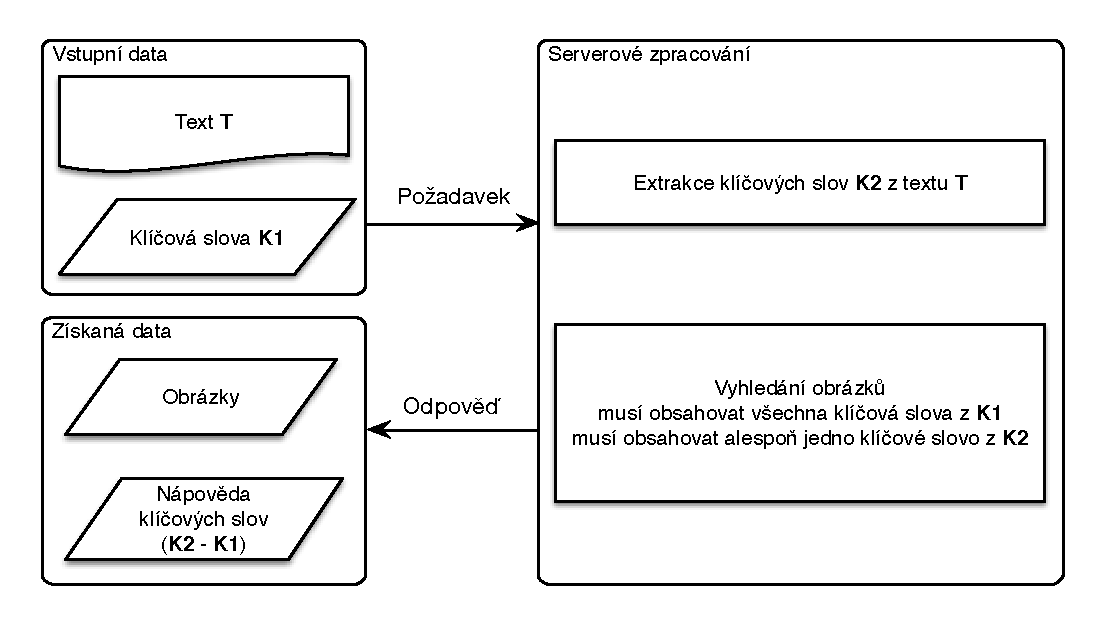
\includegraphics[width=150mm]{dataflow.eps}
  \caption{Základní tok dat mezi klientem a serverem.}
  \label{fig:dataflow}
\end{figure}


Aplikace poskytuje uživateli dvě možnosti vyhledávání. Základním uživatelským scénářem je vložit do~rozhraní text. Aplikace by v~takovém případě měla poskytnout relevantní obrázky k~danému textu. v~dalším uživatelském scénáři je přímý požadavek na klíčová slova obrázku. Uživatel by měl mít možnost zadat přímo klíčová slova, které metadata k~nalezeným obrázkům musí obsahovat. Oba scénáře by mělo navíc být možné propojit pomocí nápovědy klíčových slov -- uživatel zadá do~rozhraní text, dostane výsledné obrázky a nápovědu klíčových slov, kterými může množinu nalezených obrázků více omezit. Celý proces hledání vhodných obrázků popisuje diagram~\ref{fig:dataflow}.

\section{Extrakce klíčových slov}

Extrakce klíčových slov je velmi důležitou složkou celého vyhledávání. Článek \cite{lott} shrnuje základní techniky extrakce klíčových slov z~textu. Algoritmy na extrakci klíčových slov lze v~zásadě rozdělit do~dvou kategorií - \uv{s korpusem} a \uv{bez korpusu}. Metody pracující bez korpusu jsou zajímavé a mohou dosahovat podobných výsledků jako metody s korpusem. My však máme k~dispozici dataset Profimedie, takže o metody pracující bez korpusu se tato práce dále nezajímá. 

\section{TF-IDF}

TF-IDF\cite{tfidf} je jeden ze základních vyhledávacích algoritmů\cite{manning}. Algoritmus využívá korpusu dokumentů $D$ a dvou složek $TF$ a $IDF$, lze ho vyjádřit jako rovnost

\begin{equation}
  TFIDF(t,d,n,N)= TF(t,d)\times IDF(n,N).
\end{equation}

Složka $TF$ znamená $TERM\ FREQUENCY$ a pokud $t$ je slovo a $d \in D$ je dokument, je $TF$

\begin{equation}
 TF(t,d) = \sum_{slovo\,\in\,d} \begin{array}{l l} 1 & \mathrm{pokud}\ slovo = t \\
  0 & \mathrm{jinak} \end{array}.
\end{equation}

Jedná se tedy o frekvenci slova v~dokumentu.

Složka $IDF$, tedy $INVERSE\ DOCUMENT\ FREQUENCY$ vyjadřuje, jak moc daný termín popisuje dokument. Pokud je $N$ počet všech dokumentů v~$D$, tedy $N = |D|$ a $n$ je počet dokumentů, ve~kterých se vyskytuje slovo $t$, je $IDF$ tohoto slova

\begin{equation}
IDF(n,N) = \log \left(\frac{N}{n}\right).
\end{equation}

Čím je tedy slovo v~korpusu častější, tím více se s logaritmem snižuje jeho informační hodnota. Slova, která jsou velmi běžná, většinou klíčovými slovy nejsou.

Výsledný vzorec pak jde shrnout jako

\begin{equation}
TFIDF(t,d,n,N)= \left(\sum_{slovo\,\in\,d} \begin{array}{l l} 1 & \mathrm{pokud}\ slovo = t \\
  0 & \mathrm{jinak} \end{array}\right)
  \times
  \log \left(\frac{N - n}{n}\right).
\end{equation}

\section{TF-IDF pro~extrakci klíčových slov}
\label{sec:keywords_extraction}

Algoritmus TF-IDF můžeme použít pro~extrakci klíčových slov z~textu. Všechna znaky vstupního textu převedeme na malá písmena a text rozdělíme na slova. Odstraníme slova ze stop-slovníku, který obsahuje nejběžnější slova pro~každý z~podporovaných jazyků\footnote{Seznam slov ve~stopslovnících je převzat z~knihovny Lucene\cite{lucene}.}. Dále nás nezajímá diakritika a různé speciální znaky, které může text obsahovat.  Slova převedeme na stemy. O převodu slov na stemy se podrobněji píše v~Kapitole~\ref{chap:stemmer}.

Algoritmus TF-IDF pak použijeme na každé slovo vstupního textu a získáme tak skóre jeho významnosti v~textu. Slova s nejvyšším skóre pak označíme za~klíčová. Algoritmus musíme upravit pro~naše účely. Zaprvé nás zajímají pouze taková slova, která existují v~datasetu Profimedie. Slova, která se v~korpusu nenachází, dostanou skóre $0$. Část TF v~algoritmu znamená četnost slova v~textu.

Složitější je situace s $IDF$. Nabízí se použít frekvenci slov z~datasetu Profimedie. Ukázalo se, že klíčová slova obrázků z~datasetu nejsou pro~tento účel vhodná. Klíčová slova totiž obsahují mnoho názvů a obecně méně běžných slov. Naopak obsahují velmi málo běžných slov. To pak způsobuje, že algoritmus na tomto datasetu přiřazuje vysoké skóre běžným slovům. Tato slova ale typicky nejsou vhodnými klíčovými slovy daného textu. Je tedy potřeba použít pro~vzorec $DF$ jiný korpus. v~naší aplikaci jsme použili korpus Wikipedie\footnote{\url{http://dumps.wikimedia.org/}}, jejíž data jsou volně dostupná pro~mnoho jazyků pod otevřenou licencí.

Pokud je $w$ slovo vstupního textu, $Freq(w)$ je četnost slova ve~vstupním textu a $Wiki(w)$ je četnost slova v~korpusu Wikipedie, můžeme každému slovu vstupního slova přířadit $Score$:


\begin{equation}
  Score(w) = \left\{
  \begin{array}{l l} Freq(w) \times (\frac{C}{Wiki(w)}) & w\ \mathrm{je\ v\ datasetu\ Profimedie} \\
  0 & w\ \mathrm{není\ v\ datasetu\ Profimedie}
  \end{array}
  \right.
\end{equation}

$C$ je experimentálně zjištěná konstanta. v~našem případě je její hodnota $10\ 000\ 000$.

Nyní tedy máme skóre udávající význam slova pro~každé slovo vstupního textu. Slova s nejvyšším skóre vrátíme uživateli jako nápovědu pro~explicitní požadavek obrázků s klíčovými slovy.


\section{Vyhledávání obrázků}

Samotné vyhledávání obrázků má dva druhy vstupních dat. Prvním typem je text článku, který uživatel vloží do~uživatelského rozhraní. Máme tedy k~dispozici řetězec s textem článku. Dále může uživatel zadat explicitní klíčová slova, které má hledaný obrázek obsahovat. Tato vstupní data získáváme jako pole řetězců. Úkolem algoritmu na vyhledávání obrázků je vrátit uživateli všechny relevantní obrázky v~pořadí podle relevance.

Text si nejprve zpracujeme pomocí algoritmu uvedeném v~sekci~\ref{sec:keywords_extraction}. Získáme skóre významnosti pro~všechna slova ve~vstupním textu. pro~vyhledávání použijeme pouze několik slov s nejvyšším skóre.

Nyní můžeme jako množinu relevantních obrázků označit obrázky, které ve~svých klíčových slovech mají všechna uživatelem zadaná explicitní klíčová slova a alespoň jedno klíčové slovo získané extrakcí klíčových slov z~textu.

Množina relevantních obrázků může být velká a obsahovat obrázky, které jsou relevantní jen velmi málo. Je proto důležité množinu relevantních obrázků správně seřadit. Máme množinu $K_{text}$ klíčových slov získaných z~textu. Každé $w \in K_{text}$ má skóre $Score(w)$. Relevantní obrázek má množinu klíčových slov $K_{img}$. Relevanci obrázku vůči uživatelskému dotazu můžeme ohodnotit funkcí $Rank$:

\begin{equation}
Rank(K_{text}, K_{img}) = \sum_{w \in K_{text}}{
  \left\{
  \begin{array}{l l} Score(w) \times \frac{1}{|K_{img}|} & w\ \in K_{img} \\
  0 & w \notin K_{img}
  \end{array}
  \right.
}
\end{equation}

Vzorec bere v~úvahu počet klíčových slov, které obrázek obsahuje. Snižuje relevanci obrázků, které obsahují mnoho klíčových slov a zvýhodňuje tím ve~vyhledávání obrázky, které mají menší počet přesnějších klíčových slov.





\chapter{Překlad obrázkových popisků}

Popisky obrázků v datasetu Profimedie jsou v angličtině. Jedním z cílů aplikace je poskytnout kromě angličtiny vyhledávání i v jiném jazyce. Zaměřujeme se na češtinu, ale podobné úvahy a postupy platí většinou i pro jiné jazyky. Jsou v podstatě dvě možnosti, jak implementovat vyhledávání v češtině. Můžeme buď překládat do angličtiny hledané texty a klíčová slova, nebo předpřeložit dataset Profimedie.

My jsme se rozhodli pro druhou možnost. Musíme tedy přeložit všechny texty v datasetu Profimedie. Vzhledem k tomu, že obrázků je více než 20 milionů, nepřipadá lidský překlad v úvahu z časových i finančních důvodů. Jedinou reálnou možností je použít překlad strojový.

\section{Strojový překlad}

Strojový překlad jako obor zažívá velký rozvoj. Potřeba překladu stále celosvětově prudce stoupá. To jednak zvyšuje poptávku po kvalitním strojovém překladu a dále to strojovému překladu dává k dispozici velké množství lidských překladů, které jsou pro kvalitní strojový překlad nezbytné. Lze brát v úvahu i pravidlové překladové systémy, které ke své práci tolik dat většinou nepotřebují. Obecnější a pro většinu jazykových párů nejlepší řešení však nabízí frázový statistický strojový překlad.

\section{Frázový statistický strojový překlad}

 Frázový statistický strojový překlad\cite{koehn} ke své práci potřebuje databázi lidsky přeložených frází. Fráze jsou několikaslovné kusy přeloženého textu. Typicky se získávají z paralelního korpusu textů ve zdrojovém a cílovém jazyce. Soubor s frázovými daty obsahuje položku s textem fráze ve zdrojovém a cílovém jazyce spolu s pravděpodobností, že je takový překlad fráze správný.

Druhým důležitým vstupem strojového frázového systému je korpus cílového jazyka, ze kterého se vytvoří jazykový model. Slouží zejména k tomu, aby k sobě poskládané fráze v cílovém jazyce dobře \uv{seděly}. Pokud máme překladový i jazykový model, můžeme vyjádřit pravděpodobnost překladu pomocí základního vzorce statistického strojového překladu. Překládáme řetězec $f$ ve zdrojovém jazyce. K dispozici máme překladový model $p(f|e)$, který udává pravděpodobnost toho, že řetězec $f$ ve zdrojovém jazyce je překladem řetězce $e$ v cílovém jazyce. Jazykový model $p(e)$ nám vrací pravděpodobnost řetězce $e$ v cílovém jazyce. Chceme získat takový řetězec $\tilde{e}$, pro který je pravděpodobnost $p(e|f)$ nevyšší. Pomocí Bayesova pravidla můžeme k hledání takové fráze použít překladový a jazykový model:

\begin{equation}
 \tilde{e} = arg \max_{e \in e^*} p(e|f) = arg \max_{e\in e^*} p(f|e) p(e) 
\end{equation}

V praxi je potřeba u kvalitního strojového překladu vyřešit mnoho dalších problémů. K lepším výsledkům překladu potřebujeme reordering model, který umožňuje přesouvat pozice frází mezi zdrojovým a cílovým textem. 

Dobrý frázový překlad potřebuje ke svému chodu miliony frází. Vyhledávání nejpravděpodobnějšího překladu v takovém množství dat je náročná úloha. Algoritmy, které umožňují vyhledávat ve velkém množství překladových dat jsou implementována v knihovně Moses\cite{moses}, která je dostupná pod volnou licencí včetně základních překladových modelů pro některé jazykové páry.

\section{Charakteristika dat pro překlad}

Pro správné fungování vyhledávání v českém jazyce je potřeba přeložit klíčová slova v Profimedia datech do češtiny. Slova v korpusu jsou oddělena mezerou. Je ale zřejmé, že některá slova vedle sebe k sobě patří --- jsou to fráze --- zatímco některá nikoliv. Naskytují se tedy zhruba tři možnosti, jak takový text přeložit.


\section{Překlad vět}

\begin{figure}[h]
  \centering
  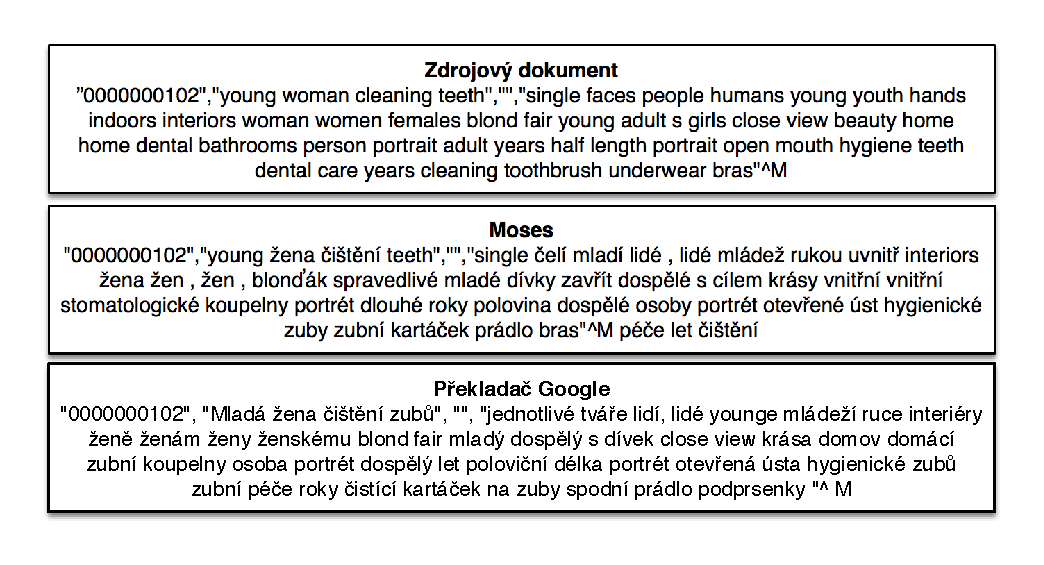
\includegraphics[width=150mm]{translate.eps}
  \caption{Ukázka překladu metadat k obrázku pomocí Mosese a Překladače Google.}
  \label{fig:translate}
\end{figure}

První možností je přistupovat k souboru klíčových slov u každého obrázku jako k větě a použít frázový strojový překlad --- buď Moses, nebo Překladač Google\cite{googletranslate} --- k překladu z angličtiny do češtiny. Tento přístup má několik problémů. Frázový překlad se snaží aplikovat fráze z překladového modelu. V našem souboru klíčových slov ale mohou být vedle sebe slova, která tvoří frázi pouze zdánlivě. Například můžeme mít fotku dítěte, které stojí před automobilem značky Seat se dvěma klíčovými slovy vedle sebe --- \uv{child} a \uv{seat}. Frázový překlad z angličtiny do češtiny pochopí tato dvě slova jako fráze, které do češtiny přeloží frází \uv{dětské sedadlo}, která ovšem neodpovídá popisku obrázku.

Dalším problémem tohoto přístupu je časová a finanční náročnost takového řešení. Frázový překlad je dosti náročný algoritmus a překlad dvaceti milionů vět může být dosti obtížný. Překlad pomocí Mosese nás omezuje výpočetní složitostí. Na jednom stroji by takový překlad trval řádově několik dní. Pokud bychom k překladu 20 milionů vět použili Překladač Google, jsme zase omezení cenou za přístup k překladovému API společnosti Google.

Pro práci s Mosesem jsme zvolili překladový a jazykový model pro překlad z angličtiny do češtiny, které jsou poskytnuty přímo s Mosesem ve verzi XX. Obrázek \ref{fig:translate} porovnává překlad metadat k jednomu z obrázků datasetu Profimedie v Mosesovi s distribuovanými překladovými daty s překladem pomocí Překladače Google. Je vidět, že Překladač Google poskytuje kvalitnější překlad. 

\section{Překlad slov}

Jednodušším přístupem k překladu klíčových slov je přístup slovníkový, tedy překlad každého slova zvlášť. Nejprve je potřeba ze souboru klíčových slov u všech obrázků vyextrahovat slova. Ty pak lze přeložit přímo s použitím slovníku, nebo pomocí frázového strojového překlad (ten použije jednoslovné fráze) Mosesem, či Překladačem Google. Výhodou oproti předchozímu přístupu je menší množství dat a tedy i nižší finanční a časová náročnost takového překladu. Takový systém překladu ale nedokáže detekovat fráze a kvalita překladu slovo od slova je typicky horší než překlad delších frází. Vezměme si například anglická slova \uv{weather} a \uv{vane}. Slovníkový překlad nám slova přeloží jako \uv{počasí} a \uv{lopatka}. Pokud se ale tato slova nachází vedle sebe, je pravděpodobnějším překladem slovo \uv{korouhvička}.

\section{Překlad frází}

Poslední možností je oba předchozí principy zkombinovat --- nejprve detekovat v souboru klíčových slov fráze a ty pak přeložit statistickým strojovým překladem. Detekci frází z datasetu Profimedia provedl ve své bakalářské práci\cite{botorek} Jan Botorek. Zkoušel detekovat N-gramy v databázi WordNet\cite{wordnet} a Wikipedii. Výsledky této detekce frází lze použít právě ke zlepšení překladu z angličtiny do cizích jazyků. Na slova, která nejsou detekována ve frázi, se použije slovníková metoda. Na překlad detekovaných frází lze použít přímo statistický strojový překlad.


\section{Řešení}

Výsledná aplikace nakonec používá poslední možnost. Bližší informace jsou v Kapitole \ref{chap:implementace}. Slova byly přeloženy pomocí Překladače Google, který překládá s lepšími výsledky než dostupný model pro překladový nástroj Moses.

Překlad frází by ovšem pomocí Překladače Google byl příliš drahý a pomocí Mosese zase příliš pomalý. Použili jsme tedy jednoduchou metodu, která používá pouze překladový model. Fráze z datasetu Profimedia byla přeložena pouze tehdy, když se její překlad nacházel v překladovém modelu. Fráze, které se v překladovém modelu nenacházely, byly přeloženy slovo od slova. Metodou přesné shody s překladovým modelem bylo přeloženo $18\ 006$ z celkového počtu $899\ 244$ detekovaných frází v Profimedia datasetu.

\section{Závěr}

Překlad klíčových slov z korpusu Profimedia není typickou překladovou úlohou --- nepřekládají se celé věty. Přesto je dokonalý výsledek nemožný. I lidští překladatelé s citem pro jazyk by v této překladové úloze dávali rozdílné výsledky. Strojový překlad zdaleka není na takové úrovni, aby dokázal z širšího kontextu vybrat správný překlad. Navíc lidský překladatel může u překladu klíčových slov využít přímo obrázek, ke kterému se klíčová slova vztahují. Může tak z obrázku posoudit, zda má slovo \uv{single} přeložit jako \uv{jednolůžkový}, nebo ve významu \uv{jeden}. Lepší překlad by mohl přinést překladový model natrénovaný na speciálnější množině dat bližší korpusu Profimedie. Vytvořit takový model by ovšem bylo nad rámec této práce.

Navrhovaný mechanismus překladu poskytuje uspokojivý, i když značně nedokonalý, překlad klíčových z angličtiny do češtiny. Jednoduše jde zevšeobecnit i pro překlad do dalších jazyků, pro které máme slovník a překladový model.


\chapter{Backend}

Moderní webové aplikace lze rozdělit na back a frontend. Backend je část aplikace, která běží na serveru. Pomocí svých služeb poskytuje přístup k databázi, k souborům uloženým na serveru a zpracovává uživatelské operace. Frontend těchto služeb využívá. Tato kapitola popisuje proces výběru backendových technologií pro tuto práci. Některé technologie se osvědčily, jiné se ukázaly pro daný účel nevhodné.

\section{Databáze}

Úkolem databáze je uložit data a umožnit jejich prohledávání. Důležitou vlastností naší aplikace je, že uživatelé nemají možnost databázi modifikovat. Zápis do databáze provede administrátor pouze jednou, před startem aplikace. Důležitým požadavkem je důraz na rychlost a snadnou škálovatelnost. V posledních letech vzniklo několik nových databází v kategorii vágně označené jako NoSQL\cite{nosql}. Tato kategorie databází se těžko popisuje, na každou popsanou vlastnost existuje NoSQL databáze, která danou vlastnost nesplňuje. Obecně ale lze říct že NoSQL databáze nepracují s prvky v tabulkovém uspořádání a oproti standardním SQL databázím nekladou tolik omezujících požadavků na data. Jejich výhodou oproti standardním relačním databázím může být vyšší výkon a snadná škálovatelnost.

Nevýhodou je většinou obtížnější práce s daty. Většina NoSQL databází například mapodporuje databázové transakce a vůbec celý ACID. Pro práci s daty v NoSQL databázi nelze použít klasické SQL dotazy. Místo nich se používá například model MapReduce\cite{mapreduce} vyvinutý ve formě Google.

První verze aplikace byla postavena na databázi CouchBase\cite{couchbase}, což je právě jedna z NoSQL databází podporující MapReduce mechanismus. Výhodou CouchBase je vysoký výkon, snadná škalovatelnost, velmi dobrá dokumentace a také existence oficiálních knihoven pro nejrozšířenější programovací jazyky. Ukázalo se však, že pro implementaci vyhledávání pro naší aplikaci je model MapReduce nedostatečný a implementace vyhledávání v CouchBase by byla prakticky nemožná.

Vhodnější pro daný účel se ukázala knihovna Elasticsearch\cite{elasticsearch}. Nejedná se v pravém smyslu o databázi. Jejím hlavním cílem je poskytnout vyhledávání nad daty. Je postavená nad knihovnou Apache Lucene ke které přidává snadnou horizontální i vertikální škálovatelnost a komunikaci pomocí REST HTTP JSON API. Díky tomu, že je Elasticsearch postaven na knihovně Lucene\cite{lucene}, může programátor využít velkou množinu možností, které Lucene poskytuje. Například v  textovém vyhledávání může využít všechny tokenizery a stemmery z knihovny Lucene. V průběhu implementace aplikace navíc vyšla stabilní verze 1.0.

\section{Programovací jazyk}

Se vzrůstající popularitou webů vzniká stále větší množství webových frameworků a dokonce programovacích jazyků zaměřených primárně na programování pro web.

\subsection{NodeJS}
Jedním z nových trendů je tvorba webového backendu v Javascriptu pomocí knihovny NodeJS. Frontendoví vývojáři jsou prakticky nucení Javascript používat. Pokud se v Javascriptu tvoří i backendová část aplikace, může snadněji dojít ke sdílení kódu i pracovních pozic. Trend psaní všech aplikací v Javascriptu glosoval již před sedmi lety Jeff Atwood ve svém pravidle:

\begin{lstlisting}
Any application that can be written in JavaScript, will eventually be written in JavaScript.
Vše co může být napsáno v Javascriptu, bude v Javascriptu napsáno.
\end{lstlisting}

Nevýhody použití Javascriptu jako backendového programovacího jazyka jsou poměrně zřejmé. Javascript byl navržen pro programování webového frontendu, jeho standartní knihovna je v porovnání s ostatními jazyky velmi chudá, podpora objektového programování je celkem nepřímočará. Obsáhlý kód v Javascriptu může být poměrně nepřehledný a jazyk svádí k vytvoření takzvaného \uv{callback hell}, který může mít strukturu jako na obrázku (source http://strongloop.com/strongblog/node-js-callback-hell-promises-generators/). Pokud chce navíc programátor sdílet kód z backendu i na frontendu, musí být kód kompatibilní s podporovanými prohlížeči. Funkce pro jednodušší práci s polem podporuje webový prohlížeč Internet Exporer až od verze 9 [http://kangax.github.io/compat-table/es5/]. V součtu nám převažily nevýhody NodeJS frameworku na výhodami a myšlenku vývoje backendu v Javascriptu jsme opustily.

\begin{lstlisting}
doAsync1(function () {
  doAsync2(function () {
    doAsync3(function () {
      doAsync4(function () {
    })
  })
})
\end{lstlisting}

\subsection{Go}

Go (známý také jako golang)\cite{golang} je programovací jazyk od společnosti Google. První stabilní verze byla zveřejněna v Květnu 2012. Go je kompilovaný, staticky typovaný jazyk s garbage collectorem. Syntaxe je inspirována jazykem C a přizpůsobena pro rychlou kompilaci. Velkou výhodou je snadná práce s vlákny pomocí \uv{go rutin}. Programátoři v Javě, nebo C++ může překvapit poněkud netypická podpora práce s objekty.

První verze aplikace byla napsána právě v jazyce Go. V praxi se ukázaly všechny výše uvedené výhody. Hlavní nevýhodou se však ukázal nedostatek kvalitních knihoven. Přestože je jazyk velmi mladý, stal se velmi populárním, o čemž svědčí například počet repozitářů na GitHubu, nebo otázek na StackOverflow. Bude to ovšem trvat ještě nějaký čas, než se knihovny pro go a jejich vývoj stabilizují. Jeden z nyní nejpopulárnějších webových frameworků pro go --- Martini --- v době začátku práce na aplikaci ani neexistoval. Právě nedostatek knihoven pro go vedl k volbě jiného jazyka. Rozhodujícím pro opuštění backendu v jazyce go byla neexistující knihovna pro práci s Elasticsearch. API je sice postaveno na protokolu HTTP, takže šlo s Elasticsearch komunikovat bez použití specializované knihovny, v praxi se to ovšem ukázalo být problematické. Vývoj aplikace si žádal testování různých nastavení a rychlé prototypování v kódu. 

Z interních zdrojů máme informaci o tom, že se Elasticsearch chystá vytvořit knihovnu i pro jazyk Go. Pro naše účely se ukázalo výhodnější přepsat aplikaci do dynamického jazyka s lepší podporou pro Elasticsearch.

\subsection{Ruby a Ruby on Rails}

Ruby je dynamicky typovaný jazyk, silně inspirovaný Perlem s důslednou podporou objektového programování. Popularita Ruby vzrostla zejména kvůli webovému frameworku Ruby on Rails, který je v Ruby napsaný. RoR zpopularizovaly koncept Model-View-Controller při tvorbě webových aplikací. Backend aplikace byl nakonec kompletně přepsán jako aplikace v Ruby on Rails. Elasticsearch poskytuje pro práci s Ruby vlastní knihovnu. Další výhodou se ukázala podpora knihovny Rake, což je jakási obdoba Makefile skriptů v Ruby. Pomocí Rakefilu jdou napsat přehledné úlohy pro manipulaci s daty. 

Standartní implementace jazyka Ruby byla v minulosti kritizována pro svou pomalost. V průběhu práce na této aplikaci vyšla verze Ruby 2.0, která Ruby dosti zrychluje. Tato rychlost byla pro aplikaci shledána dostatečnou.

\section{Komunikace frontend-backend}

Backend poskytuje služby frontendu pomocí API. Existuje několik přístupů a technologií, jak data mezi backendem a fronendem posílat.

\subsection{Formát dat}

V součastnosti jsou pro posílání dat nejběžnější dva formáty -- XML a JSON. XML je klasický formát se spoustou možností a nástrojů. Moderní aplikace však stále více přechází k formátu JSON. Formát JSON je velmi úsporný datový formát, který vychází z datových typů v JavaScriptu. Právě úspornost je jednou z jeho největších výhod oproti XML -- stejné informace mají v JSON typicky kratší zápis než obdoba v XML. Většina moderních browserů umí formát JSON parsovat a práce v JavaScriptu je pak vzhledem ke kompatibilitě datových typů velmi pohodlná.

Zejména kvůli poslednímu důvodu používá tato práce pro komunikaci mezi fronendem a backendem právě formát JSON.

\subsection{REST API}

REST je zkratka pro Representational state transfer. Jedná se o obecnou architekturu rozhraní. V tomto kontextu nás ale zajímá hlavně její navázání na protokol HTTP. REST využívá metody protokolu HTTP pro změnu, nebo získání stavu datových objektů. Ukázkou REST API s použitím formátu JSON může být například knihovna Elasticsearch. Mějme například frekvenční data pro český stem \uv{lid} a instanci Elasticsearch na adrese \lstinline{http://localhost:9200/}. Ukázky HTTP requestů XX - XX ukazují, jak taková data uložit, získat, změnit, nebo smazat.

REST API v kombinaci s JSON fromátem používá tato aplikace jak ke komunikaci mezi frontendem a backendem, tak mezi backendem a databází Elasticsearch.

\subsection{Websocket}

Alternativou k REST API a protokolu HTTP je protokol WebSocket. WebSocket je stejně jako protokol HTTP postaven nad protokolem TCP. Na rozdíl od HTTP ale poskytuje duplexní spojení. Klient je stále spojený se serverem a oba mohou posílat zprávy bez ohledu na druhou stranu. Spojení přes WebSocket má většinou menší latenci než použití protokolu HTTP \footnote{\url{http://www.websocket.org/quantum.html}}. Protokol je podporován všemi moderními verzemi webových prohlížečů a podpora existuje i v knihovnách pro backendové programovací jazyky.

První verze aplikace používali pro komunikaci mezi klientem a serverem právě protokol WebSocket. Nakonec však převážily nevýhody takovéhoto řešení nad výhodami. Jednou z nevýhod je nutnost udržovat spojení s klientem na serverové i klientské straně. Přináší to několik netriviálních problémů. Například v okamžik, kdy se toto spojení přeruší. Pokud se naproti tomu přeruší spojení server-klient při HTTP requestu, může klient zkusit vyslat stejný požadavek znovu.

Druhým problémem je emulace HTTP požadavků v protokolu WebSocket. Z klienta můžeme odeslat HTTP dotaz na server a dostaneme k němu přiřazenou odpověď. V protokolu WebSocket pošleme serveru zprávu a za nějaký čas můžeme dostat zprávu od serveru jako odpověď. Párování došlých zpráv z odeslanými zprávami-požadavky ale musíme implementovat vlastnoručně, například pomocí unikátních ID v těle zprávy. Navíc musíme umět řešit situaci, kdy žádná odpověď ze serveru nedojde. Například nastavením timeoutu pro čekání na odpověď.

WebSocket využijí zejména aplikace, které potřebují, aby server mohl posílat klientovi kdykoliv zprávy, nebo co nejnižší latenci. Takovými aplikacemi mohou být například různé chatovací služby, nebo online hry. Pro jiné většinou asi převáží nevýhody WebSockets oproti HTTP protokolu.

\section{Shrnutí}

Architektura je shrnuta na diagramu XX. Aplikace má backend napsaný v jazyce Ruby a frameworku Ruby on Rails. Data jsou uložená v databázi Elasticsearch. Backend komunikuje s frontendem i databází pomocí REST API, data jsou přenášena ve formátu JSON.









\chapter{Stemmer}
\label{chap:stemmer}

Důležitou vlastností systémů na vyhledávání v textu je, aby dokázali najít i v jiných tvarech slova. Pokud uživatel hledá slovo \uv{praha}, většinou očekává, že se mu zobrazí i výsledky obsahující slovo \uv{praze}. Je tedy potřeba mít nějaký algoritmus, který k sobě slova jako \uv{praha} a \uv{praze}.

První možností je použít lemmatizér. Úkolem lemmatizéru je ke každému slovu přiřadit jeho základní tvar. U podstatných jmen je to většinou první pád jednotného čísla (\uv{praha}), u sloves infinitiv.

Alternativou lemmatizátoru může být stemmer. Ten většinou používá jednoduché heuristiky k odstranění koncovek slov. Stemmer nemusí vrátit regulérní slovo jazyka, například pro slova \uv{praha} a \uv{praze} může stemmer vrátit slovo \uv{prah}. Výhodou stemmeru oproti lemmatizéru je, že většinou používá pouze jednoduché heuristiky. Je tedy většinou rychlejší a méně náročný na zdroje než lemmatizér. Ve vyhledávacích aplikacích je stemmer dostačující.

Pro angličtinu je nejznámějším stemmerem pro angličtinu je Porterův stemmer popsaný\cite{porter1980algorithm} Martinem Porterem již v roce 1980. Kromě oficiální implementace existují porty do různých jazyků včetně Ruby. Tato aplikace využívá implementaci z Ruby Gemu \uv{stemmify}\footnote{\url{https://rubygems.org/gems/stemmify}} v licenci MIT.


\section{Český stemmer}
Pro jazyky jako je čeština, která má bohatší morfologii než angličtina, je tvorba stemmeru náročnější. Testovali jsme několik implementací českých stemmerů. Jako nejkvalitnější byla nakonec vybrána implementace českého stemmeru v knihovně Lucene. Tuto implementaci využívá i Elasticsearch.

V rámci této práce byl portován soubor \lstinline{CzechStemmer.java} ze zdrojového kódu knihovny Lucene do jazyka Ruby. Výsledkem je Ruby Gem pod licencí MIT, který lze použít nezávisle na zbytku aplikace. Instaluje se příkazem

\begin{lstlisting}
gem install czech-stemmer
\end{lstlisting}

Knihovna obsahuje pouze jednu třídu CzechStemmer s funkcí stem, která přijímá i vrací řetězec:

\begin{lstlisting}[language=ruby]
require 'czech-stemmer'

CzechStemmer.stem("praha") # => "prah"
CzechStemmer.stem("praze") # => "prah"
CzechStemmer.stem("předseda") # => "předsd"
CzechStemmer.stem("mladými") # => "mlad"
\end{lstlisting}

\chapter{Detekce jazyka}
\label{chap:detekce_jazyka}

Aplikace může přijímat vstup ve více jazycích. Jedním ze způsobů, jak uživateli zpříjemnit práci s aplikací, je použít automatický detektor jazyka. Při zadání vstupu aplikace se aplikace sama pokusí detekovat jazyk zadaného textu. Tato detekce nemusí být vždy stoprocentně správná, takže by uživatel měl mít možnost volbu jazyka manuálně změnit.

Aplikace používá algoritmus založený na statistice nejčastějších N-gramů pro daný jazyk\cite{cavnar}. Algoritmus nejprve použije velký korpus textů pro každý detekovaný jazyk. Pro češtinu a angličtinu lze použít například korpus Wikipedie. Z tohoto korpusu získá uspořádaný seznam $K$ nejčastějších N-gramů. Při samotné detekci jazyka textu, pak samotný algoritmus získá stejný uspořádaný seznam nejčastějších N-gramů pro vstupní text. Tento seznam pak porovnává se seznamy nejčastějších N-gramů pro každý jazyk.

Nechť $A$ a $B$ jsou seznamy N-gramů s $K$ položkami, $A[w]$ je pořadí N-gramu $w$ v seznamu $A$. Potom lze vzdálenost mezi seznamy $D(A,B)$ vyjádřit vztahem:

\begin{equation}
  D(A, B) = \sum_{w\,\in\,A} \begin{array}{l l} |A[w] - B[w]| & \mathrm{pokud}\ w \in B \\
  K & \mathrm{jinak} \end{array}
\end{equation}

Na Obrázku \ref{fig:detekce_jazyka} je ukázka porovnání dvou seznamů pomocí funkce $D(A,B)$. Trigram $na\_$ se v seznamu B nenachází, proto dostane hodnotu $K = 4$.

Nyní pokud máme množinu $S$ všech seznamů N-gramů pro jednotlivé jazyky a $X$ je seznam N-gramů pro vstupní text, vrátí algoritmus jako jazyk takový jazyk, pro který má seznam $C \in S$ minimální hodnotu $D(X, C)$.


\begin{figure}[h]
  \centering
  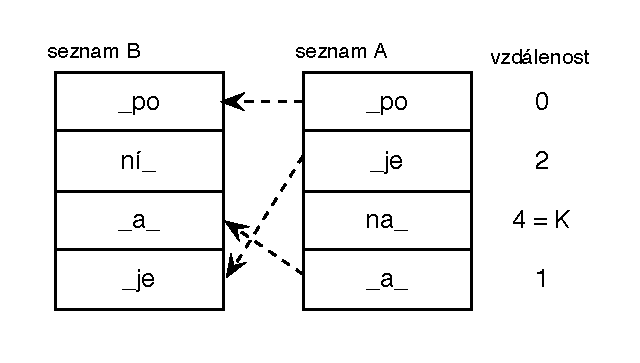
\includegraphics[width=80mm]{detekce_jazyka.eps}
  \caption{Ukázka porovnání dvou trigramových seznamů. $D(A, B) = 7$}
  \label{fig:detekce_jazyka}
\end{figure}


Naše implementace používá v seznamech N-gramů trigramy. Pro texty delší než několik slov funguje velmi spolehlivě. Pro několikaslovné texty se může stát, že v seznamu nejfrekventovanějších trigramů pro vstupní text není ani jeden trigram, který by se nacházel v seznamech pro jednotlivé jazyky. Pak algoritmus může vrátit špatně detekovaný jazyk.

Vylepšení by jistě přineslo spolu s použitím trigramů použít i bigramy a unigramy. Také konstanta $K$ by šla zvětšit z používané hodnoty $50$ výš. Implementace detekce jazyka ale probíhá na klientovi, takže všechna tato vylepšení algoritmu by zvýšila množství dat, která si klient musí stáhnout. Navíc uživatel má vždy možnost detekovaný jazyk manuálně změnit a typicky pracuje spíše s delšími texty. Implementace s použitím $50$ nejčastějších trigramů se tedy zdá dostačující pro daný účel.
\chapter{Podobné obrázky}


Jednou ze služeb, které výsledná aplikace poskytuje, je vyhledávání podobných obrázků. Uživatel rozhraní najde pomocí textových dotazů nějaké ilustrační obrázky a má možnost u každého z nalezených obrázků získat obrázky vizuálně podobné. Tato kapitola pojednává o tvorbě backendové služby, která vyhledávání podobných obrázků umožňuje.

Vstupními daty je soubor s vektory pro každý obrázek datasetu Profimedie. Vektor má $4 096$ složek s reálnými nezápornými čísly. Vektory jsou vizuální deskriptory obrázků. Tyto deskriptory byly vygenerovány pomocí software Caffe\cite{caffe} a jsou jsou odezvami předposlední vrstvy hluboké konvoluční neuronové sítě natrénované pro klasifikaci obrázků z datasetu Profimedie do 1000 kategorii.

Mějme obrázek $I_1$ s deskriptorem $D_1$ a obrázek $I_2$ s deskriptorem $D_2$. Míru podobnosti obrázků $Similarity$ pak můžeme definovat jako

\begin{equation}
  Similarity(I_1, I_2) = \sum_{i=1}^{4096} |D_1[i]-D_2[i]|
\end{equation}

V praxi se dají výsledky této míry klasifikovat zhruba do 3 kategorií. Tyto vypozorované kategorie popisuje tabulka \ref{fig:simtypes}. Ukázky jednotlivých kategorií podobných obrázků poskytuje obrázek \ref{fig:simexamples}. Rozdělení na 3 kategorie podobnosti podle míry $Similarity$ je pouze přibližné. Nelze například zaručit, že obrázek, který by některý uživatel mohl uznačit za podobný, nebude mít míru $Similarity$ vyšší než $1 500$.

\begin{figure}[h]
\label{fig:simtypes}
\centering
\begin{tabular}{ | c | r |}
  \hline
     Kategorie & $Similarity$\\
  \hline
  \hline
    téměř shodné & $0 - 500$ \\
  \hline
    podobné & $500 - 1500$ \\
  \hline
    nepodobné & $> 1500$ \\
\hline
\end{tabular}

  \caption{Kategorie podobnosti obrázků podle $Similarity$.}
\end{figure}

\begin{figure}[h]
  \centering
  \includegraphics[width=150mm]{similar_images.eps}
  \caption{Dvojice obrázků s různou kategorií podobnosti.}
  \label{fig:simexamples}
\end{figure}

Otázkou zůstává, které výsledky uživatel očekává jako výsledky vyhledávání podobných obrázků. Pravděpodobně nechce získat obrázky z kategorie \uv{nepodobné}. Pak je otázkou, jestli uživatel chce jako výsledek získat obrázky z kategorie \uv{téměř shodné}. V korpusu je spousta podmnožin obrázků, které byly vyfoceny v rámci jedné série. Často se liší jen malou změnou úhlu fotky, nebo jen kompresí uloženého obrázku. Pokud bychom vraceli obrázky seřezené podle $Similarity$, uživatelé u takovýchto podmnožit nedostanou příliš rozmanité obrázky. Vracet obrázky seřazené podle $Similarity$ tedy nemusí být vždy vhodné, náhodné pořadí obrázků z kategorií \uv{téměř shodné} a \uv{podobné} může uživatel chápat jako lepší výsledek. Tato úvaha umožňuje použít algoritmy, které nevrací obrázky seřazené podle $Similarity$, ale jsou výrazně rychlejší.


\section{Bootstrap implementace}

První implementace nahrála všechny deskriptory do databáze Elasticsearch. V Elasticsearch lze implementovat vyhledávání pomocí vlastní porovnávací funkce. Jako porovnávací funkce tedy zvolíme funkci $Similarity$. Bohužel přes některé menší optimalizace algoritmu se vyhledávání nepodařilo implementovat příliš efektivně, takže fungovalo v přijatelném čase pouze pro pár tisíc deskriptorů. Naše aplikace ovšem potřebuje pracovat s více než dvaceti miliony deskriptorů. Šly by použít další optimalizace a sharding databáze na více strojů, aby algoritmus fungoval efektivněji i na větším množství dat. To by ovšem bylo příliš drahé a navíc se objevily jiné možnosti řešení.


\section{Předgenerování výsledků}

Efektivnější variantou je ke každému obrázku vygenerovat nějaké množství podobných obrázků předem. Služba která by vracela podobné obrázky by pouze vrátila položku z databáze a neprováděla žádný výpočet. Tato služba by tak byla velmi rychlá a nenáročná na zdroje. Jako problém se ovšem ukázalo právě předgenerování obrázků. Přes snahu o co nejrychlejší implementaci v jazyce go s použitím více vláken a optimalizačních heuristik, by vygenerování podobných obrázků pro každý z 20 milionů obrázků v datasetu Profimedie trvalo na běžném počítači několik týdnů.

\section{Geohash}
Další pokus o implementaci vyhledávání podobných obrázků se inspiruje algoritmem Geohash\cite{geohash}. Algoritmus Geohash byl vyvinut v rámci služby geohash.org a jedná se o způsob zakódování prostorových dat. Jeho hlavním využitím je efektivní vyhledávání bodů (určených zeměpisnými souřadnicemi) v oblasti (na mapě). Algoritmus Geohash využívá i Google, nebo databáze Elasticsearch.

Zjednodušení algoritmu Geohash popíšeme na jednotkové podmnožině (jednotkovém čtverci) $\mathbb{R}^2$. Algoritmus postupuje tak, že čtvercovou plochu rozdělí na 4 čtverce a pojmenuje je písmeny \uv{a}, \uv{b}, \uv{c} a \uv{d}. Každý ze čtverců rekurzivně rozdělí na další čtyři čtverce, kterým dá jméno pomocí suffixů \uv{a}, \uv{b}, \uv{c} a \uv{d} k vlastnímu jména. Rekurzi provádíme do nějaké předem určené hloubky. Bodu v jednotkovém čtverci přiřadíme jméno podle čtverce s nejdelším jménem, který bod obsahuje. Každý bod v jednotkovém čtverci tedy bude mít jméno, které má stejnou délku jako hloubka rekurze. Jako oblast pak můžeme označit jakoukoliv množinu pojmenovaných čtverců. Bod leží v oblasti právě tehdy, když je jméno nějaké ho čtverce z množiny oblasti prefixem jména bodu. K ukládání názvů bodů pak lze použít prefixový strom.

Obrázek \ref{fig:geohash} ukazuje některé čtverce a jejich názvy. Pokud má algoritmus hloubku rekurze 4, má bod ležící na souřadnicích $[0.1875, 0.8125]$ název $aada$ a leží tedy ve čtvercích $a$, $aa$, $aad$ a $aada$.


\begin{figure}[h]
  \centering
  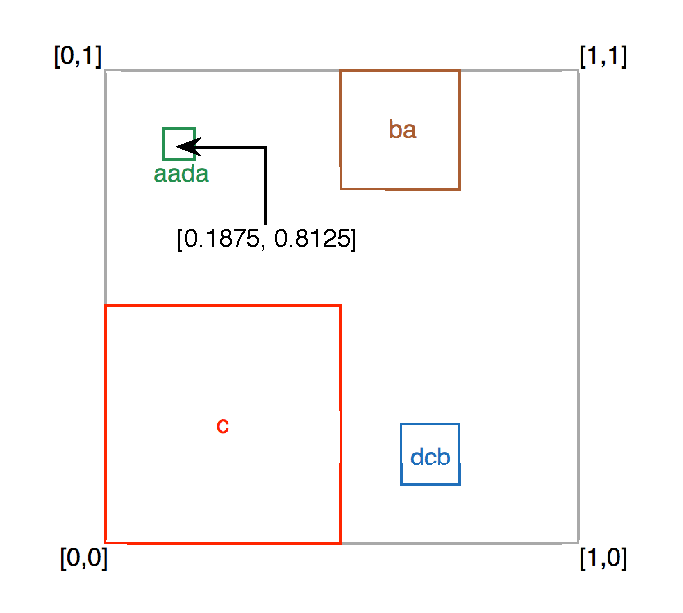
\includegraphics[width=80mm]{geohash.eps}
  \caption{Ukázka čtverců algoritmu Geohash v jednotkovém čtverci.}
  \label{fig:geohash}
\end{figure}

Nyní bychom chtěli algoritmus Geohash použít pro hledání podobných obrázků v Profimedia datasetu. Každému deskriptoru bychom nejprve přiřadily název. Množina podobných obrázků by pak obsahovala obrázky, které mají $Similarity$ s porovnávaným obrázkem nějak omezenou. Problémem je, že pomocí Geohash čtverců nedokážeme takovou oblat přesně definovat. Můžeme se ale pokusit co nejvíce oblast pomocí čtverců aproximovat. 

Pokud bychom chtěli použít Geohash pro hledání podobných vektorů přímo, narazili bychom na několik problémů. Například oblast s ohraničenou mírou $Simiarity$ nejde popsat přesně pomocí čtverců. Lze libovolně přesně aproximovat, ale s každou přesnější aproximací vzrůstá počet potřebných čtverců a zhoršuje se efektivita algoritmu. Obrázek \ref{fig:geohash_use} ukazuje jak bychom mohli použít Geohash algoritmus pro hledání podobných deskriptorů ve dvojrozměrné dimenzi. Na obrázku je popsána situace, kdy hledáme deskriptory, které mají od bodu $[0.5, 0.5]$ vzdálenost $0.5$. Tučně ohraničený čtverec vyznačuje hledanou oblast, $12$ čárkovaných čtverců tvoří aproximovanou oblast.

\begin{figure}[h]
  \centering
  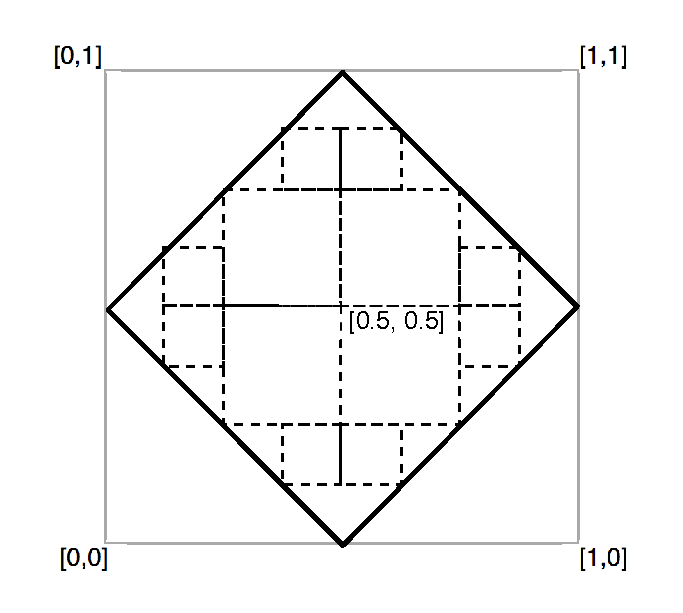
\includegraphics[width=80mm]{geohash_use.eps}
  \caption{Ukázka čtverců algoritmu Geohash v jednotkovém čtverci.}
  \label{fig:geohash_use}
\end{figure}

Ve dvou dimenzích by toto řešení fungovalo poměrně dobře. Deskriptory obrázků ovšem mají $4096$ složek a počet potřebných čtverců pro stejnou míru aproximace roste s každou dimenzí exponenciálně.

\section{Řešení}

Naše řešení využívá princip algoritmu Geohash. Jde nám o to, převést hledání podobných vektorů na fulltextové vyhledávání. Vektory reálných čísel převedeme na množinu slov oddělenou mezerami --- řetězec. Slova pochází z množiny $\{0, 1,… 4095\}$. Každé složce vektoru deskriptoru tedy odpovídá právě jedno slovo z množiny slov. Nyní přiřadíme každému deskriptoru nějakou nějakou podmnožinu slov. Způsob přiřazení je klíčovým faktorem algoritmu, který ovlivňuje jeho efektivitu. Základním způsobem je přiřadit vektoru slova, která odpovídají nenulovým vektorům. Na deskriptorech obrázků z datasetu Profimedie to znamená, že každý vektor bude mít přiřazeno zhruba 1500 slov. To je stále příliš mnoho slov pro efektivní fulltextové vyhledávání. Elasticsearch v základní konfiguraci ani neumožňuje vyhledávat s dotazy delšími než tisíc slov. Musíme tedy množinu slov dále zmenšit. Můžeme například místo nenulovosti zvýšit požadovanou mez velikosti složky vektoru.

V našem řešení používáme jinou metodu. Seřadíme složky vektorů podle velikosti a slova přiřadíme pouze $K$ složkám s nejvyšší hodnotou. Pro $K = 4$ pak každému obrázku přiřadíme řetězec, například $\mathrm{"}2013\ 432\ 1065\ 3433\mathrm{"}$. Při vyhledávání podobného obrázku nejprve získáme jeho deskriptor a jeho přiřazený řetězec. Pomocí řetězce najdeme fulltextovým vyhledáváním $L$ obrázků. Výsledky seřadíme podle podobnosti s hledaným obrázkem mírou $Similarity$ a vrátíme obrázky, které jsou v kategorii \uv{podobné}, nebo \uv{téměr shodné}. Pro správné fungování je nutné dobře nastavit hodnoty $K$ a $L$. Jejich zvýšení vede k větší přesnosti na úkor rychlosti algoritmu.

\section{Implementace}

Celá služba je implementována nezávisle na zbytku projektu. Jedná se o program \lstinline{similar_img_finder} napsaný v jazyce go. Jako databáze je použita Elasticsearch. Nejprve je nutné naimportovat data příkazem

\begin{lstlisting}
  similar_img_finder import -n 1000000 -e 9200 -k 500 -f data.gz
\end{lstlisting}

Parametr \lstinline{-n} určuje, kolik dat se má naimportovat, parametr \lstinline{-e} určuje na kterém portu běží Elasticsearch, parametr \lstinline{-k} odpovídá hodnotě $K$ a parametr \lstinline{-f} je cesta k souboru s importovanými daty.

Nyní můžeme spustit server na portu $8585$ příkazem

\begin{lstlisting}
  similar_img_finder server -p 8585 -l 100 -e 9200
\end{lstlisting}

Parametr \lstinline{-l} odpovídá hodnotě $L$.

Pokud chceme nyní získat id podobných obrázků k obrázku s id \uv{0000000003}, můžeme využít JSON HTTP API a získat výsledky na adrese \lstinline{localhost:8585/similar?id=0000000003}.






\chapter{Praktická část: Implementace moderní webové aplikace}

Práce je z velké části implementační. Snažil jsem se tedy vytvořit moderní webovou aplikaci s využitím co nejvíce frontendových novinek v novém standardu HTML5.

\section{Databáze: jak uložit 20M metadat obrázků}

Jak uložit takové množství dat, aby se dalo rychle vyhledávat. Škálovatelnost. Dostupnost knihoven pro práci s databázema. Proč jsem si vybral nakonec ES. SQL vs NoSQL.

\section{Backend a úprava dat: Komunikace s databází, implementace algoritmů}

Proč jsem zkoušel golang a proč jsem nakonec použil Ruby a Ruby on Rails. Základní popis MVC frameworku. Dostupnost knihoven pro získání stemů a prací s databází.

\section{Frontend: AJAXová aplikace na zobrazování obrázků}

Jaké jsou dnešní možnosti vývoje frontendu. Single page aplikace. Možnosti moderních prohlížečů. JavaScriptové knihovny. Proč to nedělám v jQuery, ale používám Google Closure. Google Closure Library, Templates, Compiler.

Návrh rozhraní bez jediného tlačítka. Responzivní webdesign.

\section{Anotační rozhraní}

Jak lze v Ruby on Rails vyrobit jednoduše anotační rozhraní s uživateli a s ukládáním do databáze.

\section{Návod k použití}

Popis prvků. Screenshoty aplikace.

\section{NOTES}

Language data jsem stahnul z:
http://dumps.wikimedia.org/cswiki/latest/

Ceska data jsou z:
/net/seznamdata/profiset/profi-text-cleaned.csv

prekladova data:
moses - http://www.statmt.org/moses/RELEASE-2.1/binaries/macosx-mavericks/bin/

prekladovy model:
http://www.statmt.org/moses/RELEASE-2.1/models/en-cs/

\chapter{Možnosti tvorby moderního webového frontendu}

Možnosti tvorby webových aplikací se posledních několik let rapidně zvětšují. Prohlížeče implementují stále nové technologie, které royšiřují možnosti.

\section{Možnosti programování frontendu}

Programátor webového frontendu si dnes může vybírat z několika paradigmat tvorby webové stránky. Standardem je dnes programovací jazyk Javascript. Spíše historicky bylo výhodné místo Javascriptu používat pro frontendový vývoj různé pluginy. Nejznámější je Adobe Flash, nebo Microsoft Silverlight. Programovat pro tyto pluginy mělo velké výhody. Například snadné přehrávání videa, zobrazení stránky v celoobrazovkovém režimu, nebo přístup k uživatelově webkameře. V době, kdy byla Javascriptová API velmi chudá a rozdílně implementovaná mezi prohlížeči, nabízel Flash zejména tvůrcům webových her konzistenci mezi všemi platformami.

Velkou nevýhodou těchto pluginů byla jejich proprietálnost. Ostatní firmy se bály pustit cizí plugin do svých výrobků. Zlomový moment pro ústup Flashe ze slávy bylo uvedení telefonu iPhone, který podporu pro Flash nenabízel. Softwareoví giganti Microsoft, Apple a Google začali místo proprietálních řešení tlačit otevřenou specifikaci, která se později nazvala HTML5. HTML5 je zastřešující termín pro spoustu technologií, které snaží webová API specifikovat a vytvářet nové.

\section{JavaScriptové frameworky}

Druhým hnacím motorem moderního Javascriptu jsou frameworky. Ještě před několika lety byla práce na interaktivních webech velmi náročná. Prohlížeče se zásadně lišily v implementaci práce s eventy a DOMem. Nové frameworky do jisté míry odstínily programátora od odlišných implementací Javascriptu v prohlížečích.

\subsection{jQuery}
Nejpopulárnějším frameworkem současnosti je jQuery. Ten nabízí jednoduché rozhraní a pro velkou většinu menších webových aplikací je zcela dostačující. Čím je ale aplikace větší, tím začíná být její vývoj s pomocí jQuery náročnější. Zkusme ukázat, jak by v jQuery vypadalo přidání CSS třídy red oknu s id okno:

\begin{lstlisting}
  $("#okno").addClass("red");
\end{lstlisting}

Kód má několik problémů. Pokud neexistuje žádné okno s id okno, jQuery nevrátí žádnou chybu. Stačí malý překlep a chyba v kódu se hledá dost obtížně. jQuery nenabízí žádnou funkci typu vratObjektPodleId. Pokud by tyto funkce nabízel, velikost jeho kódu by se zvětšila. Pokud chce programátor použít knihovnu jQuery, musí si ji uživatel stránky celou stáhnout. Verze XX má XX bajtů.

\subsection{Google Closure}
Jiný přístup k vývoji frontendových aplikací přináší Google. Pro svou první webovou aplikaci Gmail vyvinul sadu nástrojů, kterou později vydal jako open source pod názvem Google Closure. Kromě Gmailu ji Google využívá v Google Vyhledávání, Google Mapách, nebo Google Dokumentech. Skládá se ze tří částí - Closure Compiler, Closure Library a Closure Templates. Closure Library je obsáhlá knihovna funkcí pro práci s DOMem, Eventy, matematickými výpočty a spoustou dalších věcí, které webový programátor může využít.

Closure Compiler je inteligentní minifikátor Javascriptového kódu. Odstraňuje funkce, které nejsou volány, přejmenovává všechny názvy funkcí a proměnných na co nejkratší řetězce a v ADVANCED módu se snaží i o pokročilejší optimalizace kódu (například kód funkcí, které jsou volány pouze jednou, je vlože inline). Nejlepích výsledků dosahuje s použitím speciálních anotací, které například vynucují typ proměnné a jsou schopny udělat z Javascriptu typovaný jazyk. Closure Compiler tyto anotace vyhodnocuje a při chybném přiřazení hodnoty vrátí chybu. To umožňuje tvořit více bezpečný javascriptová kód.

Třetí částí Google Closure jsou Closure Templates, šablonovací systém pro Javascript a Javu. Pomocí Closure Templates se snadno vytváří zanořené HTML šablony. Všechny uživatelské vstupy jsou escapované což zabraňuje sniffing útokům.

Částí Templates a Compiler jdou použít odděleně v jakémkoliv Javascriptovém projektu. Používat Closure Library be Compileru nedává příliš smysl, uživatel by při návštěvě webu musel stahovat ohromné množství zbytečných dat.

Tato práce na frontendu používá všechny části knihovny Google Closure. Díky tomu si uživatel při první návštěvě webu musí stáhnout pouze jediný soubor, který má pouze XX Kb.

\section{Stylování uživatelského rozhraní a CSS}

Specifikace HTML5 rozšiřuje i možnosti vizualizace pomocí CSS stylů. Nejviditelnějšími novinkami je podpora kulatých rohů, stínování, nebo barevných přechodů. Webový programátor nyní může ke stránce načíst i vlastní font. Všechny tyto možnosti velmi rozšířily možnosti webovým grafikům.








\chapter{Instalace a zprovoznění}

Celé anotační rozhraní je webová aplikace napsaná v jazyce Ruby a frameworku Ruby on Rails. Je k dispozici pod svobodnou licencí MIT. K jejímu spuštění potřebujete ruby verze alepoň 2.0 (nižší verze nejsou otestované), javu a ke stažení zdrojového kódu git. Program jde spustit na Linuxu a Macu.

\section{Instalace}

Zdrojový kód je volně dostupný na webu GitHubu\footnote{\url{https://github.com/hypertornado/diplomka}}. Stáhnou tedy lze příkazem

\begin{lstlisting}[language=bash]
git clone https://github.com/hypertornado/diplomka
\end{lstlisting}

Tento příkaz vytvoří adresář diplomka. Závislosti aplikace nainstalujete pomocí bundleru:

\begin{lstlisting}[language=bash]
bundle install
\end{lstlisting}

Instalace může vyžadovat přístup administrátora. Dále je potřeba stáhnout knihovnu elasticsearch\footnote{\url{http://www.elasticsearch.org/downloads/1-0-3/}} do adresáře bin/elasticsearch. Stačí verze 1.0 a vyšší. Ve verzi 1.2.1 jsme objevili menší chybu\footnote{\url{https://github.com/elasticsearch/elasticsearch/issues/6611}}, která je způsobena chybou v Javě a jde obejít nastavením delšího hostname počítače.

Nyní je možné celý projekt spustit. Nejprve se spustí elasticsearch databáze pomocí příkazu \lstinline{rake es:start}, poté je možné spustit samotnou aplikaci příkazem \lstinline{rails server}. Po spuštění severu je uživatelské rozhraní dostupné ve webovém prohlížeči na adrese \lstinline{http://localhost:3000}. Po načtení stránky se zobrazí uživatelské rozhraní, ale veškeré AJAXové dotazy skončí chybou. V databázi nejsou importována data.

\section{Práce s metadaty k obrázkům}

Metadata k obrázkům a obrázky samotné jsou poskytovány firmou Profimedia a nejsou volně dostupné. Ke zprovoznění aplikace je nutné vložit CSV soubor \lstinline{keyword-cleaned-phrase-export.csv} do adresáře data.

\section{Překlad metadat}
Soubor obsahuje metadata k obrázkům v angličtině. Jedním z úkolů této práce je poskytnout doporučování obrázků i v jiných jazycích, primárně v českém jazyce. Bylo tedy nutné metadata přeložit. Pokoušeli jsme se použít volný nástroj na překlad Moses. Ve verzi 2.1\footnote{\url{http://www.statmt.org/moses/RELEASE-2.1/models/en-cs/model/}} nabízí volně dostupné modely pro překlad z češtiny do angličtiny. I na SSD disku trvá několik hodin, než se překladový model načte do paměti. Překlad jednoho segmentu s tímto modelem byl poměrně pomalý (překlad metadat k jednomu obrázku trval zhruba 3 sekundy) a také dosti nepřesný. Například řádek

\begin{lstlisting}
"0000000003","little baby smiling","","child children baby babies infants kids childhood single faces body naked nake facial expressions smile smiling viewing watching laying fun amusing amusement amused amuse dallying frolicing playing wantoning open"^M
\end{lstlisting}

byl do čestiny přeložen takto:

\begin{lstlisting}
"0000000003","little|UNK|UNK|UNK dítě smiling","","child|UNK|UNK|UNK dětí , dětské děti kojence děti dětství jednotného čelí orgán nahé nake|UNK|UNK|UNK pořídili vyjádření usmívat usmívá odůvodněním , která zábavné sledovat zábavné zábavných i pobavena tím amuse|UNK|UNK|UNK dallying|UNK|UNK|UNK frolicing|UNK|UNK|UNK hrát wantoning|UNK|UNK|UNK open"^M|UNK|UNK|UNK
\end{lstlisting}

Je vidět poměrně velké množství nepřeložených slov (koncovky \lstinline{|UNK}) a překlad je relativně nepřesný. Je pravděpodobné, že by s lepšími daty šel natrénovat lepší překladový a jazykový model. Strojový překlad není hlavním tématem této práce, takže bylo jednodušší komerční automatický překlad Google Translate, který přeloží ukázková metadata takto:

\begin{lstlisting}
"0000000003", "malé dítě s úsměvem", "", "dítě děti dítě děti kojenci děti dětství jednotlivé plochy těla nahá nake výrazy obličeje, úsměvu, usměvavý sledování sledování kterým zábava zábavné zábavní pobavený pobavit laškoval frolicing hrát wantoning otevřený" ^ M
\end{lstlisting}

I z této ukázky je zřejmé, že Google poskytuje kvalitnější překlad, než anglicko-český překladový model v releasu Mosese. Google poskytuje překlad zdarma přes webové rozhraní. Pokud se ale do překladového formuláře nahraje nespecifikované větší množství dat, přestane překlad fungovat. Google pro překlad poskytuje placené API. Platí se XX amerických dollarů za přeložené slovo. Korpus Profimedie obsahuje zhruba (wc vystup 20119222 347129204 4811998848), takze by cely překlad stál XX dollaru. Jelikož se slova v textu opakuji, lze použít překlad slovo po slovu. Ještě lepší by bylo překládat přímo klíčové fráze. Bohužel korpus Profimedie jednotlivé fráze neodděluje. Je ale možné použít učící algoritmus a klíčové fráze detekovat.

\subsection{Export slov a frází}
Nejprve příkazem \lstinline{rake data:export_profimedia_words_for_translation} vyexportujeme do souboru \lstinline{data/word_list.txt} seznam všech slov použitých v metadatech k obrázkům. Tento příkaz běží několik hodin i na moderním počítači s SSD diskem. Z Profimedia dat získáme seznam 352862 slov. Tento soubor je nutné přeložit z angličtiny do dalších podporovaných jazyků, v našem případě češtiny.

\section{Jazykový korpus}
Tato práce potřebuje jazykové korpusy pro podporované jazyky ze dvou důvodů. První je potřeba pro určení relativní jazykové frekvence slov v algoritmu TF-IDF. Zadruhé je potřeba jazykový korpus pro rozpoznávání jazyků. Přirozeným jazykovým korpusem by mohla být samotná Profimedia data, ale pro oba účely jsou tato data nepoužitelná. Klíčová slova a názvy obrázků jsou odlišnými druhy textů, než je průměrný článek. Je tedy potřeba jazyková data získat jinde.

Wikipedia se jako korpus velmi hodí. Textový obsah je pod licencí Creative Commons a jeho struktura je velmi podobná běžnému publicistickému článku. Data se dají získat stažením přímo ze serverů wikipedie (pro češtinu zde), nebo pomocí sdílených torrentů. Práce wiki dumpy všech podporovaných jazyků v adresáři data pod názvem typu \lstinline{wiki_dump_jazyk.xml}. Pro práci s daty z wikipedie je potřeba nejprve převést XML data do textového formátu. K tomu slouží python skript \lstinline{lib/WikiExtractor.py} od Wikipedie. Pro převod anglických dat lze použít příkaz:

\begin{lstlisting}
rake wiki:extract_words_from_wiki en
\end{lstlisting}

Stejný příkaz je potřeba spustit i pro ostatní podporované jazyky. Příkaz vytvorí v \lstinline{data/wiki_en} adresářovou strukturu. Není potřeba převést všechna data, pouze tolik, abychom dostali reprezentativní korpus. Pro angličtinu stačí převést zhruba 10000 článků, pro podobné množství českých dat je potřeba převést zhruba 20000 článků (údaj o exportovaných článcích je průběžně vypisován na konzoli).

Nyní je možné vytvořit seznam slov v korpusu s frekvencemi. Ve skutečnosti nás zajímají pouze stemy slov, ne jednotlivé tvary. Příkaz

\begin{lstlisting}
rake wiki:frequency_list_from_wiki
\end{lstlisting}

vytvoří seznam slov a jejich frekvencí s cestou \lstinline{data/wiki_freq_list_count.en}. Ve skutečnosti nás nezajímají všechna slova z korpusu wikipedie, ale pouze ta, která se vyskytují mezi klíčovými slovy v Profimedia korpusu. Příkazem

\begin{lstlisting}
rake data:create_tf_df_list
\end{lstlisting}

se z korpusu profimedia dat exportují stemy všech slov v profimedia korpusu spolu z hodnotami udávajícími frekvenci termínu v celém korpusu (TF) a frekvenci toho, v kolika popiskách obrázků se slovo objevilo (DF). Pro angličtinu jsou tato data uložena do souboru \lstinline{data/tf_df_list_en.txt}. Nyní můžeme spárovat informaci o stemech z wikipedie a nahrát je do databáze. Párování se provede příkazem:

\begin{lstlisting}
rake data:pair_profimedia_and_wiki_data
\end{lstlisting}

který vytvoří soubor \lstinline{data/paired_wiki_and_profimedia.txt} se statistikami všech stemů z Profimedia korpusu.


\section{Příprava dat pro detekci jazyků}

Automatická detekce jazyka probíhá ve frontendové části. Ke svému chodu ale potřebuje data z korpusu, konkrétně seznam nejčastějších trigramů pro každý podporovaný jazyk. Příkaz

\begin{lstlisting}
rake trigrams:extract_most_frequent_trigrams
\end{lstlisting}

vytvoří pro každý jazyk seznam padesáti nejčastějších trigramů. Seznam pro angličtinu je uložen v souboru \lstinline{data/most_frequent_trigrams_en.txt}. Příkaz

\begin{lstlisting}
rake trigrams:trigrams_to_javascript_classes
\end{lstlisting}

pracuje se seznamy nejčastějších trigramů ze kterých vytvoří javascriptovou třídu \lstinline{oo.diplomka.Languages.Data} v notaci Google Closure. Ta je uložena v souboru \lstinline{public/js/js/diplomka/languages/data.js}.

\section{Import dat do databáze}

Veškerá data jsou importována do databáze elasticsearch. Aplikace očekává Elasticsearch připojený na portu 9200. Samotná data se importují příkazem:

\begin{lstlisting}
rake es:import_image_metadata
\end{lstlisting}

Tento vytvoří v elasticsearch index diplomka. Poté nastaví explicitní mapování v celém indexu. Pokud se mapování explicitně nenastaví, elasticsearch se snaží data namapovat podle jednoduchých heuristik. Například text rozdělí na slova, která pak převede na malá písmena a upraví defaultním stemmerem. Aplikace se však o stemming a převedení na malá písmena stará sama, mapování tedy říká, aby nahraný text oddělil pouze pomocí mezer na slova a dále nezpracovával. Vyhledávací dotaz je pak rozdělen také pouze pomocí mezer. Nastavené mapování lze ověřit pomocí API elsaticsearch na adrese \url{http://localhost:9200/diplomka/_mapping/}.

Po vytvoření indexu může začít samotný import dat. Data z každého řádku Profimedia dat je převeden do formátu JSON. Data obsahují položky locator, title 

\section{Import metadat obrázků}





\chapter{Anotační rozhraní}

Vrámci této práce bylo implementováno anotační rozhraní pro vyhodnocování algoritmů, které přiřazují vhodné obrázky k textům. Anotační rozhraní je velmi univerzální. Anotátor má ve webové aplikaci v levém sloupci novinový text a v pravém sloupci galerii obrázků. Jeho úkolem je označit obrázky, které se k danému textu hodí a obrázky které se k textu nehodí. Má také možnost nechat obrázek neoznačený, pokud by se nemohl rozhodnout ani pro jednu variantu.

\section{Instalace rozhraní}

Celé rozhraní je aplikace napsaná v jazyce Ruby a frameworku Ruby on Rails. Aplikace je volně šiřitelná pod licencí MIT. Pro zprovoznění anotační aplikace je potřeba UNIXový systém (Linux, Mac). Zdrojový kód aplikace je uložen na severu GitHub\footnote{\url{https://github.com/hypertornado/cemi_anotace}} a nejlépe jde stáhnout pomocí gitu. Pro běh serveru je potřeba verze ruby 2.0 a vyšší. Celá aplikace se zprovozní následujícím pořadím BASH příkazů:

\begin{lstlisting}[language=bash]
git clone https://github.com/hypertornado/cemi_anotace
cd cemi_anotace
bundle install #nainstaluje vsechny ruby zavislosti
rake db:migrate #vytvori sqlite databazi s tabulkami
rails server #spusti anotacni server na portu :3000
\end{lstlisting}

\section{Přidání uživatelů}

Po spuštění serveru je možné přidat anotátory \href{http://localhost:3000/users}{v administračním rozhraní}. Přístup je zaheslován HTTP autentifikací. Defaultní uživatelské jméno je cfo a heslo cfo85. Administrátorské přístupové údaje lze změnit v souboru \lstinline{ROOT_APLIKACE/app/controllers/admin_controller.rb}. Uživatelé mají pouze dvě datové položky, uživatelské jméno (Name) a heslo (Password). Uživatele jde přidávat, mazat a upravovat. Nepředpokládá se, že by anotovaná data byla vysoce citlivá, heslo je proto v databázi uloženo v plaintextu.

\section{Import anotačních dat}

Data pro anotaci lze nahrát pomocí příkazu

\begin{lstlisting}[language=bash]
rake data:import
\end{lstlisting}

Příkaz očeká existenci souboru \lstinline{ROOT_APLIKACE/public/annotation_inputs.csv}. Ten musí mít speciální formát, kdy je každý řádek rozdělen mezerami na šest sloupců s následujícími položkami:

\begin{description}

\item[INDEX] \hfill \\
  unikátní číslo jedné anotace
\item[LABEL] \hfill \\
 interní popis pokusu
\item[PRIORITY] \hfill \\
 priorita, celé číslo $>= 0$. Určuje prioritu s jakou se má anotace přiřadit. Čím vyšší číslo, tím vyšší priorita.

\item[PREFER\_USER] \hfill \\
 uživatelské jméno preferovaného anotátora. Pokud není žádný anotátor preferován, použije se pomlčka
\item[TEXT\_FILE] \hfill \\
 cesta k textovému souboru s referenčním článkem
\item[IMAGE\_FILES] \hfill \\
 seznam cest k obrázkům. Cesty nemohou obsahovat mezery a jsou oddělené středníkem.
\end{description}

Ukázka importovaných dat:

\begin{lstlisting}[language=bash]
1 basics 0 - ./text/aha/aha-00263.txt.gz  img/1.jpg;img/2.jpg;img/3.jpg
2 basics 1 - ./text/aha/aha-00006.txt.gz  img/1.jpg;img/2.jpg
3 basics 0 - ./text/aha/aha-00009.txt.gz  img/2.jpg
\end{lstlisting}

\section{Export anotačních dat}

Hotové anotace lze exportovat příkazem

\begin{lstlisting}[language=bash]
rake data:export
\end{lstlisting}

Tento příkaz vypíše na konzolu řádky, které mají tabulátorem oddělené položky:

\begin{description}

\item[INDEX] \hfill \\
  ID anotace. Stejné jako u importovaných dat.
\item[USER] \hfill \\
  Jméno anotátora, který anotaci vytvořil.
\item[TIME] \hfill \\
  Čas uložení hotové anotace ve formátu UNIX timestamp.
\item[SKIPPED] \hfill \\
  Pokud uživatel anotaci přeskočil, je hodnota True, jinak False.
\item[APPROPRIATE] \hfill \\
  Seznam obrázků které anotátor označil jako vhodné k textu ve formátu relativních cest oddělených středníkem.
\item[NOT\_APPROPRIATE] \hfill \\
  Seznam obrázků které anotátor označil jako nevhodné k textu ve formátu relativních cest oddělených středníkem.

\end{description}

\section{Import obrázků a textů}

Anotační texty a obrázky musí být nahrány do adresáře \lstinline{ROOT_APLIKACE/public} tak, aby jejich cesty odpovídali cestám v souboru \\ \lstinline{ROOT_APLIKACE/public/annotation_inputs.csv}. Pokud tedy importovaný soubor obsahuje cestu k obrázku \lstinline{img/1.jpg}, musí být nahrán odpovídající soubor do \lstinline{ROOT_APLIKACE/public/img/1.jpg}.

Obrázky musí být ve formátu, který podporují webové prohlížeče, tedy hlavně JPEG a PNG. Texty musí být uloženy v textových souborech s kódováním utf-8 a komprimovaný pomocí gzip\footnote{\url{http://www.gzip.org/}}.




\chapter{Testování výsledků}
\label{chap:evaluace}

Výsledný program se skládá z~několika komponent. Funkčnost každé komponenty lze testovat. Některé části je možné otestovat automaticky, například rozpoznávání jazyka. Na některé části je potřeba testování s uživateli.

Klíčovou částí celého projektu je algoritmus, který k~textu přiřadí ilustrační obrázek. Úspěšnost tohoto algoritmu byla otestována na uživatelích. Rozhraní může fungovat pro~více jazyků. Testování však proběhlo pro~vstupní texty v~češtině. Výhodou je snadnější získání anotátorů v~českém jazyce. Hlavním důvodem je ovšem pravděpodobná vyšší nepřesnost algoritmu v~češtině. Dataset Profimedie má data v~anglickém jazyce a pro~české použití musel být přeložen. Pokud se tedy ukáže, že algoritmus funguje dobře pro~češtinu, měl by pro~angličtinu fungovat ještě lépe. pro~testování bylo využito testovací rozhraní popsané v~Kapitole~\ref{chap:rozhrani}.


\section{Vyloučení narušitele (o\_test1)}

\begin{figure}[h]
  \centering
  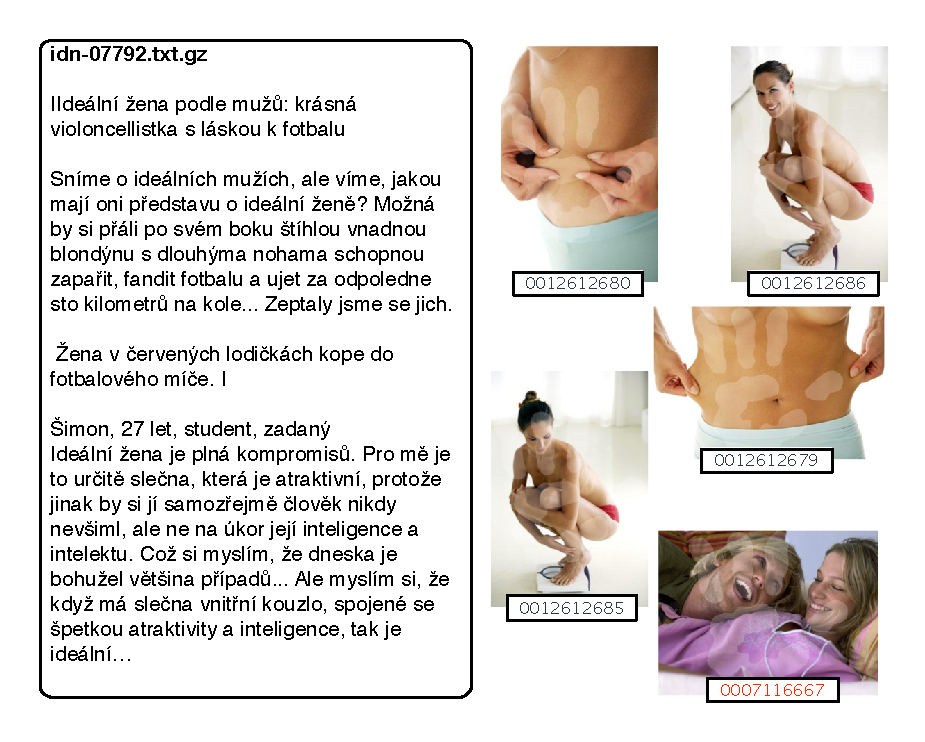
\includegraphics[width=150mm]{evaluace_1.eps}
  \caption{Ukázka testu vyloučení narušitele pro~článek idn-07792.}
  \label{fig:evaluace_1}
\end{figure}


První metodou testování bylo \uv{vyloučení nepřítele} (anglicky \uv{intruder detection}). Tato metoda se používá k~evaluaci automaticky detekovaných shluků slov a je popsána například v~\cite{chang}. v~naší variantě se evaluují obrázky přiřazené k~textu. Nejprve se k~danému textu najdou pomocí testovaného algoritmu 4 nejvíce odpovídající obrázky. k~nim se přidá jeden náhodně vybraný obrázek z~datasetu a poté se náhodně zamíchá pořadím těchto obrázků. Anotátor vidí v~anotačním rozhraní text a 5 obrázů. Jeho úkolem je označit obrázek, který danému textu podle jeho názoru odpovídá nejméně. Pokud algoritmus přiřazující obrázky textu funguje správně, měl by být uživatel schopen označit obrázek, který byl do~sady vybrán náhodně a rozlišit ho od obrázků, který vybral algoritmus přiřazující obrázky.

Texty pro~testování algoritmu pochází z~korpusu online článků stažených z~českých webových serverů. Jedná se o články, které obsahují ilustrační obrázky z~datasetu Profimedie. Takto omezená množina novinových textů je pro~náš účel velmi výhodná. pro~různé druhy článků dataset Profimedie neobsahuje žádné vhodné ilustrační obrázky. Jedná se například o politické zpravodajství, pro~které v~datasetu aktuální fotky událostí nebo například archivní fotky osobností. Oproti tomu u článků, které již nějaký ilustrační obrázek z~Profimedie obsahují, jsou možnosti vhodného obrázku daleko vyšší. Jedná se většinou o hobby a společenské články.

Pro naše testování jsme využili články ze serveru iDnes\footnote{\url{http://www.idnes.cz}}, který obsahoval nejvíce článků s ilustračními obrázky z~Profimedia. Konkrétně jich máme k~dispozici $4223$.

Z těchto $4 223$ článků jsme náhodně vybrali pro~testování 60 článků. Ke každému z~článků byly získány algoritmem 4 doporučené ilustrační obrázky a byl přidán jeden obrázek náhodný. Každá tato testovací sada byla otestována dvěma anotátory. Bylo k~dispozici 5 anotátorů. Dohromady to znamenalo pro~každého anotátora 24 a dohromady 120 anotací. Anotace byly rozděleny tak, aby každá dvojice anotátorů měla právě 6 stejných testovacích sad.

Během anotace se zjistilo, že u dvou testovacích sad se jeden z~obrázků nenačítá. Tyto sady byly z~testování vyřazeny a anotovaných testovacích sad je tedy pouze 58. Výsledky testování jsou shrnuty v~tabulce~\ref{tab:testresults} ve~sloupci \uv{o\_test1}. Pobrobné výsledky testování včetně Cohenovy kappy pro~všechny dvojice anotátorů jsou v~příloze~\ref{app:testing}.

Výsledky ukazují, že pro~78~\% testovacích sad měli anotátoři pozitivní shodu. Pozitivní shoda znamená, že se oba anotátoři shodli na stejném obrázku, který je pro~vstupní text nejméně vhodný. Tento obrázek byl zároveň vybrán do~testovací sady náhodně. Čím je toto procento vyšší, tím lépe náš algoritmus pracuje, protože uživatelé jsou schopní detekovat náhodný obrázek. pro~5~\% testovacích sad máme negativní shodu. Oba anotátoři vybrali obrázek, který nebyl přiřazen náhodně. Znamená to tedy, že tento obrázek nebyli schopní detekovat a algoritmus tedy pro~vstupní text nepracuje dobře (pokud vyloučíme možnost, že náhodně přiřazený obrázek je k~textu relevantní). U poslední skupiny testovacích dat -- 17~\% -- byl pouze jeden z~anotátorů schopen vybrat náhodně vybraný obrázek. 

\begin{table}
\label{tab:testresults}
\centering
\begin{tabular}{ | l || r | r | r |}
  \hline
     & \multicolumn{1}{c |}{\textbf{o\_test1}} & \multicolumn{1}{c |}{\textbf{o\_test2}} & \multicolumn{1}{c |}{\textbf{celkem}} \\
  \hline
  \hline
    \textbf{anotátorů} & 5 & 5 & 7 \\
  \hline
    \textbf{textů} & 58 & 120 & 178 \\
  \hline
    \textbf{anotací} & 116 & 240 & 356 \\
  \hline
    \textbf{pozitivní shoda} & $45/58=78\%$ & $76/120=\mathbf{63}\%$ & $121/178=67\%$ \\
  \hline
    \textbf{negativní shoda} & $3/58=5\%$ & $15/120=13\%$ & $18/178=10\%$ \\
  \hline
    \textbf{neshoda} & $10/58=17\%$ & $29/120=24\% $ & $39/178=22\%$ \\
\hline
\end{tabular}

  \caption{Přehled výsledků uživatelského testování.}
\end{table}

Získaná data ukazují, že algoritmus pracuje poměrně správně. Pokud by algoritmus přiřazoval automaticky obrázky k~textům i v~praxi, čtenáři by byli schopní výstupy tohoto algoritmu odlišit od algoritmu, který přiřazuje obrázky k~textům náhodně.

Během testování se objevil jeden zásadní problém s testovací metodou. v~datasetu Profimedie jsou i obrázky, které jsou si velmi vizuálně podobné, například fotky stejné osoby z~různých úhlů. Tyto fotky mají často i stejné textové popisky. Mějme tedy 4 obrázky, které jsou si vizuálně velmi podobné a mají stejné textové popisky. Pokud algoritmus označí jako nejvhodnější obrázek k~textu jeden z~těchto obrázků, budou i na dalších třech doporučených pozicích vizuálně podobné obrázky (pokud tedy nemáme jinou množinu obrázků, která má stejné textové popisky, ale je vizuálně odlišná). Pokud se takový text objeví v~naší testovací metodě, uvidí anotátor 4 velmi podobné obrázky a k~nim jeden náhodně vybraný. Nejméně vhodný obrázek pak snadno označí, aniž by vůbec četl anotační text. Ukázalo se, že v~našem testování k~takovému problému opravdu došlo -- anotátorovi se zobrazily obrázky, z~nichž ani jeden nebyl vhodným obrázkem k~danému textu, přesto anotátor snadno označil nejméně vhodný obrázek. Tento problém může zkreslovat výsledky testování touto metodou.

Dobře je tento problém vidět na ukázce anotace v~Obrázku~\ref{fig:evaluace_1}. Text článku je anketa mezi muži o ideální ženě. Obrázek ze sady fotek s tématem hubnutí by asi nebyl úplně ideální ilustrační obrázek k~danému článku. Možná že náhodně přidaný obrázek s~id \uv{0007116667} by článek ilustroval lépe. Oba anotátoři ho však označili za~nejméně vhodný, protože ostatní obrázky jsou ze stejné série.

Zajímavé je analyzovat, proč obrázky s tématikou hubnutí přiřadil algoritmus jako vhodné k~článku o ideální ženě. Algoritmus v~článku označil jako klíčová postupně slova \uv{ideální}, \uv{žena}, \uv{let}, \uv{svobodný} a \uv{ráda}. První nalezený obrázek má id \uv{0012612680}. Slovo \uv{ideální} se v~českém překladu nachází dvakrát (z překladu frází \uv{ideal figure} a \uv{ideal body measurements}). Dvakrát se v~klíčových slovech obrázku nachází \uv{žena}. Stejně tak slovo \uv{let} z~anglického \uv{years}, které není pro~daný obrázek příliš relevantní. Slovo \uv{svobodný} se do~českých metadat obrázku dostalo nesprávným překladem. Anglická metadata obrázku obsahují frázi \uv{skin folds upper body freely}. Slovo \uv{freely} by v~takovém kontextu mělo být přeloženo spíše jako \uv{volný} než jako \uv{svobodný}. Obrázek s id \uv{0012612680} ukazuje velkou část problémů, které algoritmus vyhledávání ilustračních obrázků k~textu má, zejména s přeloženými texty.


\section{Detekce správného obrázku (o\_test2)}

Abychom předešli problémům s metodou popsaným v~předchozí sekci, provedli jsme nové testování. Úkolem uživatelů bylo nyní vybrat obrázek, který se ke vstupnímu textu hodí nejvíce. Množinu obrázků nyní tvořil jeden výstup z~algoritmu a 4 náhodně vybrané obrázky. Zvětšili jsme i testovací sadu. Bylo testováno 120 textů náhodně vybraných z~iDnes datasetu. Každý z~textů byl anotován dvěma anotátory. Na každém z~pěti anotátorů tedy bylo 48 anotací. Výsledky testování jsou shrnuty v~Tabulce~\ref{tab:testresults} ve~sloupci \uv{o\_test2}. Pobrobné výsledky testování, včetně Cohenovy kappy pro~všechny dvojice anotátorů je v~příloze~\ref{app:testing}.

Výsledky jsou oproti předchozí metodě o něco horší. pro~63~\% testovacích sad měli oba anotátoři pozitivní shodu, pro~13~\% měli anotátoři negativní shodu a pro~24~\% se anotátoři neshodli.

Zajímavý je rozbor anotací, u kterých správný obrázek neuhodl ani jeden z~obrázků. Některé nesprávně označené výsledky jsou způsobeny špatnou volbou náhodných obrázků. v~anotaci textu \uv{idn-01911} ukázané na Obrázku~\ref{fig:evaluace_2_1} o~novém softwarovém centru společnosti Microsoft se náhodně objevili 3 obrázky na kterých je počítač.

\begin{figure}[h]
  \centering
  \includegraphics[width=130mm]{evaluace_2_1.eps}
  \caption{Obrázky v~evaluaci textu idn-01911. Algoritmem doporučený je 2. obrázek v~pořadí.}
  \label{fig:evaluace_2_1}
\end{figure}


Podobný problém má anotace na Obrázku~\ref{fig:evaluace_2_1}, kde se u článku o úbytku plochu polí a zvětšování plochy lesů objevily náhodně obrázky pole a lesa. Tyto problémy při testování algoritmu by šly odstranit lepším výběrem náhodných obrázků. Například by obrázky mohly být náhodně vybrány z~množiny, která neobsahuje žádné z~doporučených klíčových slov textu.

\begin{figure}[h]
  \centering
  \includegraphics[width=130mm]{evaluace_2_2.eps}
  \caption{Obrázky v~evaluaci textu idn-02505. Algoritmem doporučený je 4. obrázek v~pořadí.}
  \label{fig:evaluace_2_2}
\end{figure}

Někdy jsou špatné výsledky způsobeny chybným nastavením důležitosti jednotlivých klíčových slov. Obrázek~\ref{fig:evaluace_2_3} ukazuje obrázky u anotace článku o povýšení a kariéře žen. Algoritmus pro~detekci klíčových slov správně určil jako první klíčové slovo \uv{ženy}. Na dalších pozicích jsou \uv{manažerských}, \uv{muže}, \uv{řídících} a \uv{zaměstnání}. Doporučený obrázek kromě klíčového slova \uv{ženy} obsahuje všechna ostatní detekovaná klíčová slova. Anotátoři však měli ve~výsledcích obrázek se ženou, kterému dávali přednost.

\begin{figure}[h]
  \centering
  \includegraphics[width=130mm]{evaluace_2_3.eps}
  \caption{Obrázky v~evaluaci textu idn-04282. Algoritmem doporučený je 3. obrázek v~pořadí.}
  \label{fig:evaluace_2_3}
\end{figure}


Problémem se ukázaly být také příliš krátké popisky obrázků. Obrázek~\ref{fig:evaluace_2_4} ukazuje anotační obrázky pro~text vracení záloh za~elektřinu. Třetí obrázek má v~klíčových slovech jediné slovo \uv{backup}, které je přeloženo jako \uv{záloha}. Vyhledávací algoritmus preferuje ve~výsledcích obrázky s kratšími popisky klíčových slov, takže se tento obrázek s jednoslovným popisem stal doporučeným k~danému textu. Zdá se z~více případů, že tyto obrázky s velmi krátkými popisky by mohly být pro~lepší výsledky z~vyhledávání odstraněny.

\begin{figure}[h]
  \centering
  \includegraphics[width=130mm]{evaluace_2_4.eps}
  \caption{Obrázky v~evaluaci textu idn-04368. Algoritmem doporučený je 3. obrázek v~pořadí.}
  \label{fig:evaluace_2_4}
\end{figure}

\section{Shrnutí}

Uživatelské testování ukazuje, že je algoritmus schopen v~poměrně velkém procentu případů přiřadit automaticky \uv{dostatečňě vhodný} ilustrační obrázek. To, že je ilustrační obrázek dostatečně vhodný ovšem neznamená, že je nejvhodnější. Výběr nejvhodnějšího ilustračního obrázku je ovšem velmi individuální a nedá se obecně měřit. Při testování se ukázalo, že některé náhodně vybrané obrázky, byly anotátory označeny jako lepší ilustrační obrázky pro~daný text, než obrázky automaticky přiřazené algoritmem. To ovšem neznamená, že by tyto obrázky byly vždy pro~daný test nevhodné. Ukazuje se, že některé druhy textů mohou obsahovat poměrně širokou škálu přijatelných ilustračních obrázků.

Testování ukázalo také na slabiny algoritmu. Možná největší slabinou je fáze překladu, díky níž popisky k~některým obrázkům nesprávné. Tímto problémem netrpí algoritmus pro~anglické vyhledávání, který pracuje s nepřeloženými popisky. Další množina problémů je způsobena nesprávnými popisky u obrázků. Některé obrázky jsou popsány desítkami klíčových slov, jiné zase pouze jedním.

Jedním z~problémů našeho testování je omezená doména testovaných textů. Můžeme říci, že algoritmus funguje dobře na nějaké doméně textů, ale pro~obecné zpravodajské články může algoritmus fungovat velmi špatně. Toto ovšem není problém testovaného algoritmu, ale dat, na kterých pracuje. Rozšíření domény obrázků v~korpusu Profimedie by rozšířilo i doménu textů, pro~které algoritmus funguje dobře.

%problemy: idn-00881.txt.gz - rise vinnetoua plitvice










% Ukázka použití některých konstrukcí LateXu (odkomentujte, chcete-li)
%%%% Ukázka použití některých konstrukcí LaTeXu

\subsection{Ukázka \LaTeX{}u}
\label{ssec:ukazka}

V~této krátké části ukážeme použití několika základních konstrukcí \LaTeX{}u,
které by se vám mohly při psaní práce hodit.

Třeba odrážky:

\begin{itemize}
\item Logo Matfyzu vidíme na obrázku~\ref{fig:mff}.
\item Tato subsekce má číslo~\ref{ssec:ukazka}.
\item Odkaz na literaturu~\cite{lamport94}.
\end{itemize}

Druhy pomlček:
červeno-černý (krátká),
strana 16--22 (střední),
$45-44$ (minus),
a~toto je --- jak se asi dalo čekat --- vložená věta ohraničená dlouhými pomlčkami.
(Všimněte si, že jsme za~\verb|a| napsali vlnovku místo mezery: to aby se
tam nemohl rozdělit řádek.)

% Makro na české uvozovky (novější verze LaTeXu ho už mají zabudované)
\newcommand{\uv}[1]{\quotedblbase #1\textquotedblleft}
\uv{České uvozovky.}

\newtheorem{theorem}{Věta}
\newtheorem*{define}{Definice}	% Definice nečíslujeme, proto "*"

\begin{define}
{\sl Strom} je souvislý graf bez kružnic.
\end{define}

\begin{theorem}
Tato věta neplatí.
\end{theorem}

\begin{proof}
Neplatné věty nemají důkaz.
\end{proof}

\begin{figure}
	\centering
	
\includegraphics[width=30mm]{../img/logo.eps}
	\caption{Logo MFF UK}
	\label{fig:mff}
\end{figure}


\chapter{Závěr}
\addcontentsline{toc}{chapter}{Závěr}

Podařilo se nám implementovat webovou aplikaci pro~vyhledávání ilustračních obrázků z~textu. Obrázky pochází z~datasetu Profimedie. Každý obrázek má přiřazena klíčová slova, která aplikace používá k~vyhledávání. Podporuje český a anglický jazyk, ale je snadno rozšiřitelná na podporu jiných jazyků. Uživatel může nejen zadat text článku, ale může si i vynutit přímo klíčová slova u hledaných obrázků.

Klíčovým algoritmem pro~vyhledávání je algoritmus extrakce klíčových slov. Ten je založen na modifikované metodě TF-IDF. Extrahovaná klíčová slova se používají k~vyhledávání doporučených obrázků. Druhé využití vyextrahovaných klíčových slov z~textu je jako nápověda uživateli.

Zdrojová data v~datasetu Profimedia jsou v~angličtině. Aby aplikace byla schopná pracovat s českými texty, bylo nutné klíčová slova obrázků přeložit. Použili jsme hybridní metodu, která kromě slovníkového překladu využívá i překlad detekovaných víceslovných frází v~textu. Menší kvalita takového překladu způsobuje občasné problémy algoritmu při doporučování obrázků k~českým textům. Při tak velkém množství dat by ovšem kvalitnější překlad byl velmi náročný~na zdroje, nebo příliš drahý.

Součástí práce je i rozbor některých moderních možností tvorby frontendu a backendu webových aplikací. Práce vysvětluje některé novinky v~HTML5 a ukazuje využití javascriptových frameworků pro~různé účely. Na backendové straně aplikace ukazuje některé nové komunikační a datové protokoly. Rozebrány jsou některé možnosti uložení velkého množství prohledavatelných dat.

Kromě textového vyhledávání umožňuje aplikace i vyhledávání podle vizuální podobnosti obrázků. Uživatel aplikace vidí v~detailu každého z~nalezených obrázků množinu podobných obrázků. v~rámci aplikace byla vytvořena nezávislá služba, která k~obrázkům v~datasetu Profimedia hledá obrázky. Podobnost obrázků je určena vzdáleností vektorů se $4\ 096$ složkami. Jelikož obrázků v~datasetu Profimedia je více než 20 milionů, bylo největším úkolem implementovat službu doporučování obrázků tak, aby vracela kvalitní výsledky co nejrychleji.

Algoritmus doporučování ilustračních obrázků byl testován s lidskými anotátory. Anotátoři dostávali české texty z~online médií a množinu obrázků. Některé obrázky byly získané algoritmem na doporučení obrázků k~textu. Jednu anotaci dostali nezávisle na sobě vždy dva anotátoři. v~prvním úkolu dostali anotátoři jeden náhodný a čtyři doporučené obrázky. z~58 anotací označili anotátoři správně náhodně vybraný výsledek ve~45 případech. Ukázalo se ovšem, že metoda testování má některé problémy, které umožnily anotátorům vybrat náhodný obrázek aniž by ostatní obrázky byly k~textu relevantní. Druhá metoda testování otočila poměr a anotace obsahovaly čtyři náhodné a jeden doporučený obrázek. Úkolem anotátorů bylo označit právě jeden nenáhodný obrázek. Každou anotaci opět dostali nezávisle na sobě vždy dva anotátoři. Ze 120 anotací se oba anotátoři shodli na správném obrázku v~76 případech. Rozbor anotací u kterých se oba anotátoři neshodli ukazuje různé příčiny. Některá klíčová slova k~obrázkům jsou chybně přeložena. Některé obrázky obsahují špatná klíčová slova. Klíčová slova některých obrázků jsou příliš krátká. v~několika anotacích by některé z~náhodně vybraných obrázků mohly být ilustrační obrázky k~textu také, což negativně ovlivnilo výsledky testování v~neprospěch algoritmu. pro~anglické články testování neproběhlo, ale je pravděpodobné, že dosažené výsledky by byly lepší --- u anglických klíčových slov nebylo potřeba použít automatický překlad.

Testování ukázalo, že aplikace ve~vysokém procentu nabízí uživatelům přijatelné ilustrační obrázky. Pokud jsou výsledky nevyhovující, může uživatel využít nápovědu doporučených klíčových slov a hledaný výsledek snadno přesněji specifikovat. ve~výsledku by tedy aplikace měla být schopna usnadnit proces vyhledávání ilustračních obrázků ke zpravodajským článkům, což bylo hlavním cílem práce.



%%% Seznam použité literatury
%%% Seznam použité literatury je zpracován podle platných standardů. Povinnou citační
%%% normou pro diplomovou práci je ISO 690. Jména časopisů lze uvádět zkráceně, ale jen
%%% v kodifikované podobě. Všechny použité zdroje a prameny musí být řádně citovány.

\def\bibname{Seznam použité literatury}
\begin{thebibliography}{99}
\addcontentsline{toc}{chapter}{\bibname}

\bibitem{lamport94}
  {\sc Lamport,} Leslie.
  \emph{\LaTeX: A Document Preparation System}.
  2. vydání.
  Massachusetts: Addison Wesley, 1994.
  ISBN 0-201-52983-1.

\bibitem{porter80}
  {\sc Porter,} Martin F.
  \emph{An algorithm for suffix stripping}.
  Program: electronic library and information systems, 1980, 14.3: 130-137



\end{thebibliography}


%%% Tabulky v diplomové práci, existují-li.
\chapwithtoc{Seznam tabulek}

%%% Použité zkratky v diplomové práci, existují-li, včetně jejich vysvětlení.
\chapwithtoc{Seznam použitých zkratek}

%%% Přílohy k diplomové práci, existují-li (různé dodatky jako výpisy programů,
%%% diagramy apod.). Každá příloha musí být alespoň jednou odkazována z vlastního
%%% textu práce. Přílohy se číslují.
\chapwithtoc{Příloha 1}
\label{app:testing}
\lstinputlisting[]{annotation_results.txt}


\openright
\end{document}
